\documentclass{article}
\usepackage[italian]{babel}
\usepackage{hyperref}
\usepackage{graphicx}
\usepackage{float}
\usepackage[x11names,table]{xcolor}
\usepackage{array}
\usepackage[margin=3cm]{geometry}
\graphicspath{ {./imgs/} }

\title{VezGammon - Report finale Team 1 \\ \large Progetto di Ingegneria del Software}
\author{Lorenzo Peronese - Scrum Master}

\begin{document}

\maketitle

\tableofcontents

\newpage

\section{Descrizione del prodotto}
\subsection{Introduzione}
Per il progetto del corso di Ingegneria del Software, il team ha scelto di lavorare a VezGammon\textsuperscript{\texttrademark}, 
un'applicazione web di backgammon. Il progetto ha diversi riferimenti alla città di Bologna, in cui è nato e si è sviluppato: 
in primis ovviamente il nome (\textit{"vez"} viene usato a Bologna come intercalare e significa amico, fratello); inoltre una 
volta nel sito il cursore diventa un simpatico tortellino e la board utilizza i colori rosso e blu, rappresentativi della città.

L'applicazione offre un'esperienza di gioco completa con diverse modalità: gli utenti possono sfidarsi in partite locali sullo 
stesso dispositivo, mettere alla prova le proprie abilità contro intelligenze artificiali di vari livelli di difficoltà e confrontarsi 
online con altri giocatori attraverso un sistema di matchmaking o mediante link di invito diretti. È inoltre possibile organizzare 
tornei a quattro partecipanti, combinando liberamente giocatori reali e bot di diversa difficoltà.

Il sistema di classificazione si basa sul metodo Elo, ampiamente utilizzato negli scacchi. Ogni nuovo account parte da una base 
di 800 punti, che vengono poi aggiornati dopo ogni partita online o torneo. Il calcolo dell'aggiornamento tiene conto di diversi 
fattori: l'esito della partita, l'utilizzo del dado double e il punteggio Elo di entrambi i giocatori. Questo sistema garantisce 
una competizione equilibrata e permette di mantenere una classifica globale, dove ogni giocatore può aspirare a raggiungere le 
posizioni più alte.

VezGammon\textsuperscript{\texttrademark} include anche ricche funzionalità social e di progressione. Gli utenti possono consultare 
(e condividere sui social) in ogni momento statistiche dettagliate delle proprie partite, visualizzare grafici che mostrano l'andamento 
del proprio Elo nel tempo e analizzare i match recenti. Il sistema premia inoltre i giocatori con speciali badge al raggiungimento 
di specifici obiettivi, come vincere un determinato numero di partite o raggiungere certi livelli di punteggio Elo, aggiungendo 
un ulteriore elemento di coinvolgimento e progressione al gioco.

\subsection{Backlog} \label{sec:bl}
\begin{figure}[H]
    \centering
    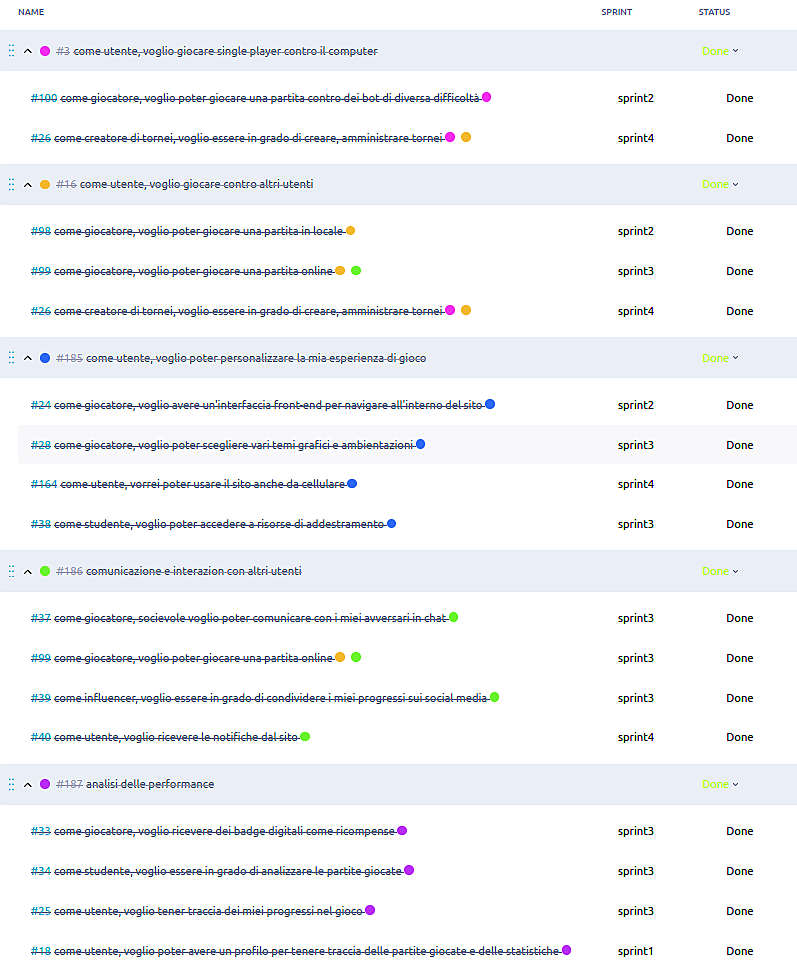
\includegraphics[width=1\textwidth]{backlog}
    \caption{Backlog di Taiga di Vezgammon\textsuperscript{\texttrademark}}
    \label{fig:backlog}
\end{figure}

\subsection{UML}
\subsubsection{Casi d'uso}

\vspace{70pt}

\begin{figure}[H]
    \centering
    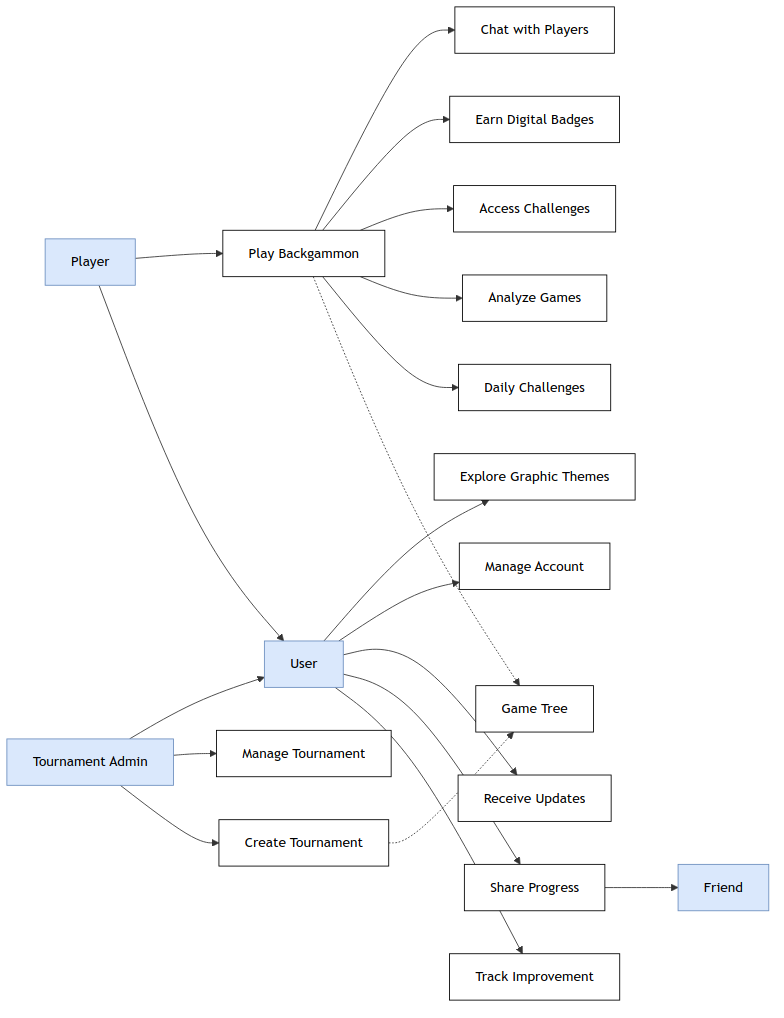
\includegraphics[width=16cm]{uml-usecase}
    \caption{Diagramma UML use-case}
    \label{fig:use-case}
\end{figure}
\subsubsection{Deployment}
\begin{figure}[H]
    \centering
    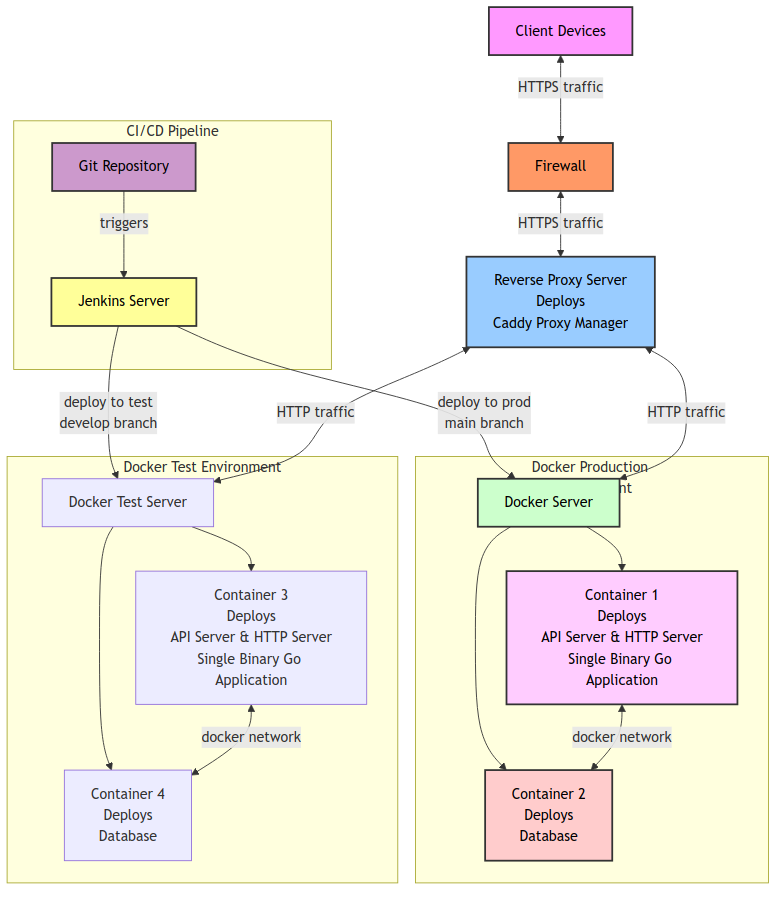
\includegraphics[width=1\textwidth]{uml-deployment}
    \caption{Diagramma UML di deployment}
    \label{fig:deployment}
\end{figure}
\subsubsection{Classi}
\begin{figure}[H]
    \centering
    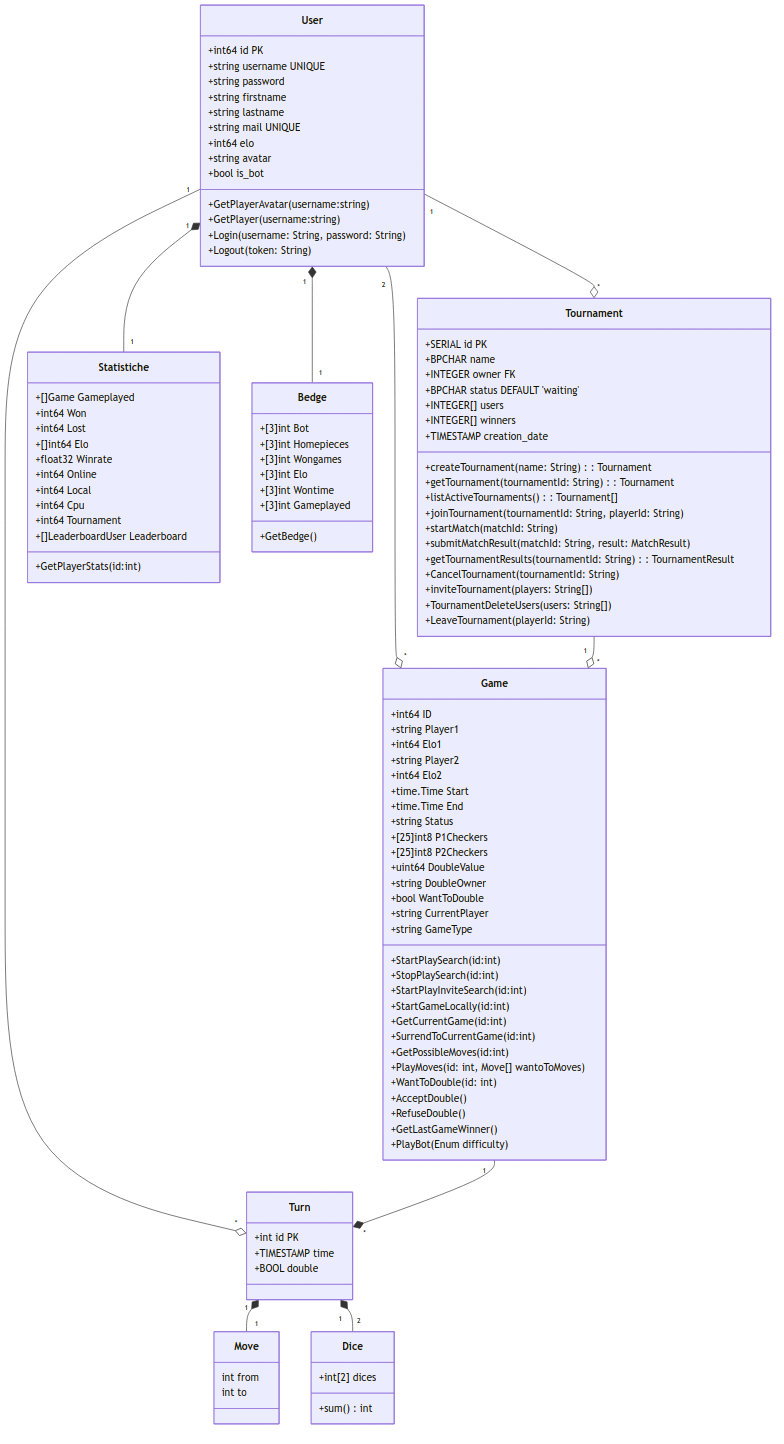
\includegraphics[width=14cm, height=19cm]{uml-classes}
    \caption{Diagramma UML delle classi}
    \label{fig:class-diagram}
\end{figure}

\section{Infrastruttura e tecnologia utilizzata}

\subsection{CAS: ambiente di sviluppo agile}

Il team ha adottato un approccio completamente open-source, basandosi sull'ambiente CAS consigliato dai docenti. 
Tutti i software sono stati self-hostati sotto il dominio \href{https://vezgammon.it}{\texttt{vezgammon.it}} per garantire 
un controllo completo sui dati e per avere meno dipendenze possibili con l'esterno. Questo ha inizialmente richiesto 
un notevole sforzo ma a lungo termine sono emersi i benefici di questa scelta.

Le credenziali di accesso sono state fornite agli stakeholder al momento della creazione dell'infrastruttura ma possono 
essere resettate su richiesta.

\subsubsection{GitLab}
GitLab è stato utilizzato per la gestione del codice sorgente e per il versioning. Sono stati utilizzati i tag per denotare 
il Minimun Value Product di ogni sprint. 
Qui è stato creato il repository, gestito le merge request e segnalato e risolto le issue.

Il repository è accessibile all'indirizzo \href{https://gitlab.vezgammon.it}{\texttt{gitlab.vezgammon.it}}  

\subsubsection{Taiga}
Taiga è stato scelto per la gestione del project management. È stato utilizzato per tracciare le attività, gestire il 
backlog (vedi \ref{sec:bl}), definire le user stories e monitorare lo stato di avanzamento del progetto durante gli sprint.

Il progetto Taiga è accessibile all'indirizzo \href{https://taiga.vezgammon.it}{\texttt{taiga.vezgammon.it}}

\subsubsection{MatterMost}
Come descritto nella Sezione \ref{sec:mm}, MatterMost è stato utilizzato per la comunicazione interna del team. È stata 
la piattaforma principale per gli scambi di messaggi, la condivisione di aggiornamenti e per accordarsi sugli incontri quotidiani.

MatterMost self-hosted è accessibile all'indirizzo \href{https://mattermost.vezgammon.it}{\texttt{mattermost.vezgammon.it}}

\subsubsection{Jenkins}
Jenkins è stato utilizzato come \textit{core} per l'automazione del flusso di lavoro tramite CI/CD e dei processi di build 
e deployment. Sono stati configurati job automatici per costruire, testare e distribuire l'applicazione.

Jenkins self-hosted è accessibile all'indirizzo \href{https://jenkins.vezgammon.it}{\texttt{jenkins.vezgammon.it}}

\begin{figure}[H]
    \centering
    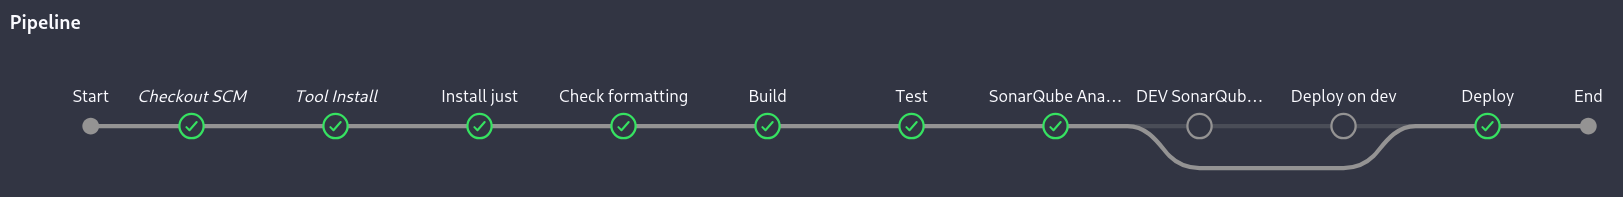
\includegraphics[width=1\textwidth]{report-jk_pipeline}
    \caption{Pipeline di Jenkins: viene lanciata a ogni evento push su GitLab e controlla formattazione, build e test; sui 
    commit delle branch \textit{main} e \textit{develop} viene anche eseguito il controllo statico del codice con SonarQube 
    e il deploy sul relativo server, di produzione o di sviluppo.}
    \label{fig:jk_pipeline}
\end{figure}

\subsubsection{SonarQube}
Come descritto nella Sezione \ref{sec:sq}, SonarQube è stato utilizzato per l'analisi della qualità del codice. \'E stato 
configurato SonarQube per eseguire analisi statiche e rilevare eventuali problematiche riguardanti la qualità del codice, 
la copertura dei test e la manutenzione.

SonarQube self-hosted è accessibile all'indirizzo \href{https://sonarqube.vezgammon.it}{\texttt{sonarqube.vezgammon.it}}

\subsubsection{Swagger} \label{sec:swagger}

Per la documentazione delle API implementate e il testing più rapido è stato utilizzato il tool 
\textit{Swagger}(\url{https://swagger.io/}). \\
Vengono di seguito riportate alcune immagini che ne illustrano il funzionamento.

\begin{figure}[H]
    \centering
    \begin{minipage}[t]{0.48\textwidth}
        \centering
        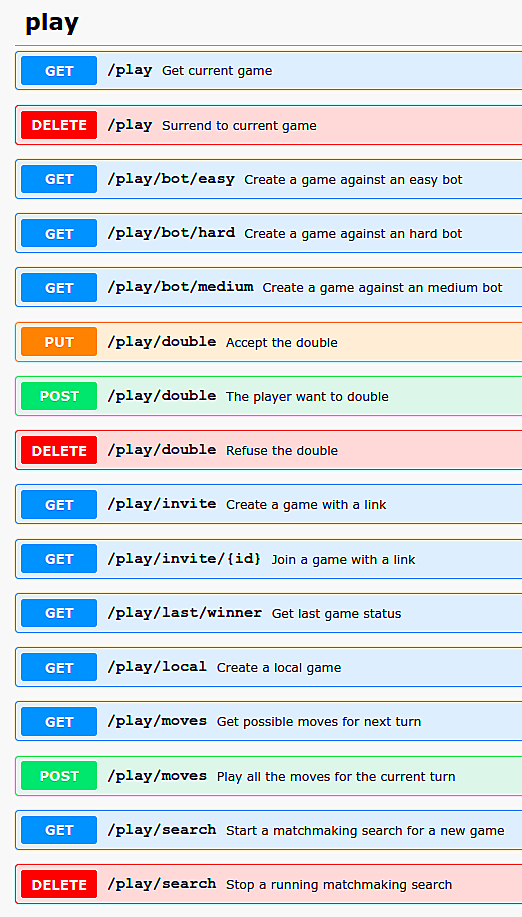
\includegraphics[width=\textwidth]{report-sw_overview}
        \caption{API utilizzate per gestire una generica partita}
        \label{fig:sw_overview}
    \end{minipage}
    \hfill
    \begin{minipage}[t]{0.49\textwidth}
        \centering
        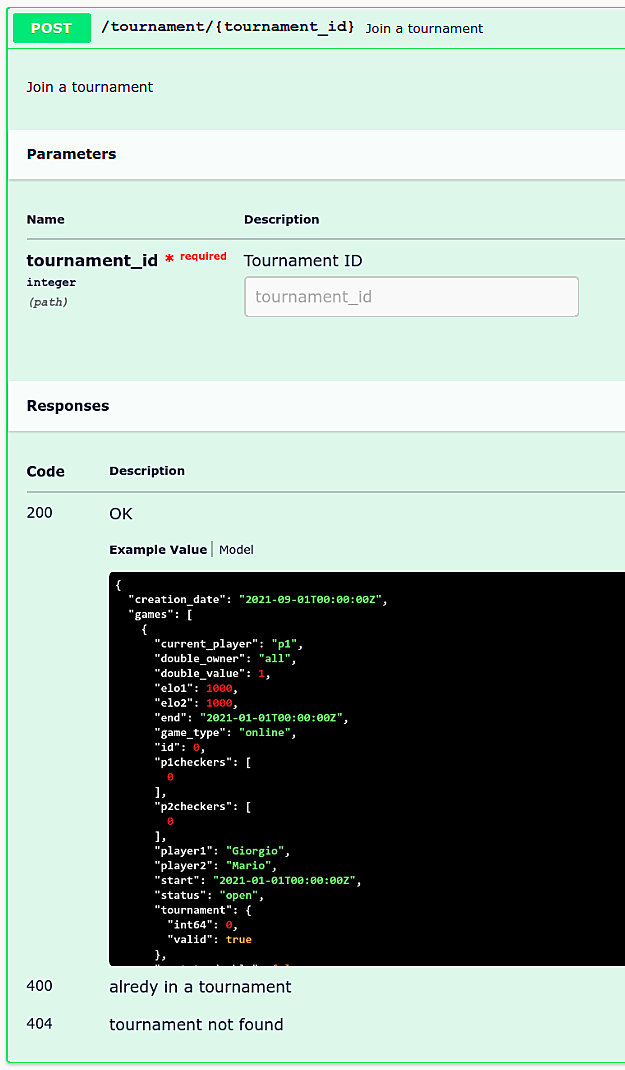
\includegraphics[width=\textwidth]{report-sw_joinTournament}
        \caption{Nel dettaglio, l'interfaccia di Swagger per ogni API}
        \label{fig:sw_joinTournament}
    \end{minipage}    
\end{figure}

\newpage

\subsubsection{Status}
\label{sec:status}
È stato configurato un sistema di monitoraggio dei servizi interamente open-source per tenere traccia della disponibilità 
dei vari strumenti utilizzati nel progetto.

\'E stato inoltre integrato con un bot Telegram per avvisare tempestivamente di eventuali problemi con il server 
e/o i singoli servizi.

Il sito che riassume lo stato dei servizi è accessibile all'indirizzo \href{https://status.vezgammon.it}{\texttt{status.vezgammon.it}}

\subsubsection{bgweb-api}
Il team ha utilizzato \href{https://github.com/foochu/bgweb-api}{\texttt{bgweb-api}} come software open-source di validazione delle mosse, 
un wrapper del software utilizzato da \texttt{GNU-Backgammon} compatibile con il linguaggio Go.

\subsection{Stack Web}

\paragraph{Frontend}
\begin{itemize}
    \item \textbf{Framework}: \href{https://github.com/vuejs/core/}{\texttt{Vue.js}}
    \item \textbf{Libreria di styling}: \href{https://github.com/tailwindlabs/tailwindcss}{\texttt{Tailwind CSS}}
\end{itemize}

\paragraph{Backend}
\begin{itemize}
    \item \textbf{Linguaggio}: \href{https://github.com/golang/go}{\texttt{Go}}
    \item \textbf{Framework}: \href{https://github.com/gin-gonic/gin}{\texttt{Gin}}
\end{itemize}

\paragraph{Database}
\begin{itemize}
    \item \textbf{Tipo}: \href{https://github.com/postgres/postgres}{\texttt{PostgreSQL}}
    \item \textbf{Interfaccia web}: \href{https://github.com/sosedoff/pgweb}{\texttt{Pgweb}}
\end{itemize}

\paragraph{Comunicazione}
\begin{itemize}
    \item \textbf{Architettura}: \texttt{REST API}
    \item \textbf{Documentazione}: \texttt{Swagger} (vedi \ref{sec:swagger})
\end{itemize}

\paragraph{Deploy}
\begin{itemize}
    \item \textbf{Containerizzazione}: \href{https://github.com/docker}{Docker}
    \item \textbf{Proxy HTTP}: \href{https://github.com/caddyserver/caddy}{Caddy}
\end{itemize}

\subsection{Server di gioco}

Sono stati configurati due server principali per ospitare l'applicazione:
\begin{itemize}
    \item \textbf{Server di produzione}: \href{https://vezgammon.it}{\texttt{vezgammon.it}}
    \item \textbf{Server di sviluppo}: \href{https://dev.vezgammon.it}{\texttt{dev.vezgammon.it}}
\end{itemize}
Il server di produzione è stato utilizzato per la versione stabile, mentre il server di sviluppo è stato dedicato al testing, 
al debug e alle fasi di sviluppo continuo.

\section{Descrizione del processo}

Il team ha deciso di comune accordo e su richiesta del \textit{Product Owner} di dedicare al progetto quattro sprint di due settimane 
ciascuno, in aggiunta allo sprint 0, dedicato alle attività di teambuilding e alla familiarizzazione con l'ambiente di sviluppo, e 
al release sprint, in cui il focus è andato su risoluzione dei bug, qualità del codice e stesura di questo report finale.

\subsection{Il team}

\begin{itemize}
    \item \textbf{Product Owner}: Diego Barbieri
    \item \textbf{Scrum Master}: Lorenzo Peronese
    \item \textbf{Full-stack Developer + DevOps}: Samuele Musiani
    \item \textbf{Frontend Developer}: Emanuele Argonni
    \item \textbf{Backend Developer}: Fabio Murer
    \item \textbf{Backend Developer}: Omar Ayache
\end{itemize}

Il gruppo è composto da sei membri ed è la prima volta che lavoriamo tutti insieme su un progetto di questa portata. Sebbene non ci 
conoscessimo tutti a vicenda inizialmente, alcuni di noi avevano già collaborato durante precedenti attività, sia universitarie 
che non. Durante gli sprint abbiamo avuto modo di approfondire la conoscenza reciproca in un contesto diverso dal solito, rafforzando 
il rapporto e favorendo una collaborazione più efficace.

Prima di iniziare lo sprint 0, il team si è riunito di persona per definire i ruoli; questi sono stati rispettati per la maggior parte, 
ma con un approccio flessibile: lo Scrum Master e il Product Owner hanno aiutato nello sviluppo del frontend, mentre il developer full-stack
si è spostato tra frontend e backend in base alle necessità dello sprint. Questa versatilità ha permesso di ottimizzare il lavoro 
e affrontare le sfide che si sono presentate in modo più efficace.

\subsection{Teambuilding} \label{sec:teambuilding}

Durante lo sprint 0, in due giornate diverse, sono state organizzate le due attività di teambuilding: \textit{Scrumble} e 
\textit{Escape The Boom!}.

Il primo gioco, \textit{Scrumble}, si è rivelato inizialmente complicato da comprendere; tuttavia, una volta avviata l'attività, i membri 
del team hanno rapidamente preso il ritmo. Nonostante gli obiettivi prefissati del gioco non siano stati minimamente raggiunti, l'esperienza 
si è rivelata piacevole e coinvolgente. Il gruppo ha avuto l'opportunità di familiarizzare con la metodologia Scrum, un "assaggio" pratico 
di come funziona il lavoro in sprint.

Il secondo gioco, \textit{Escape The Boom!}, è stato più intuitivo da avviare ma non meno impegnativo. Il team si è suddiviso in due gruppi: 
il primo era incaricato di leggere e interpretare le istruzioni, mentre il secondo aveva il compito di disinnescare la bomba virtuale. Anche 
in questo caso, il gruppo ha trascorso un'ora divertente e stimolante, sebbene con risultati altrettanto modesti.

Di seguito la tabella dell'autovalutazione di \textit{Scrumble}, compilata da tutti i partecipanti:

\begin{figure}[H]
    \centering
    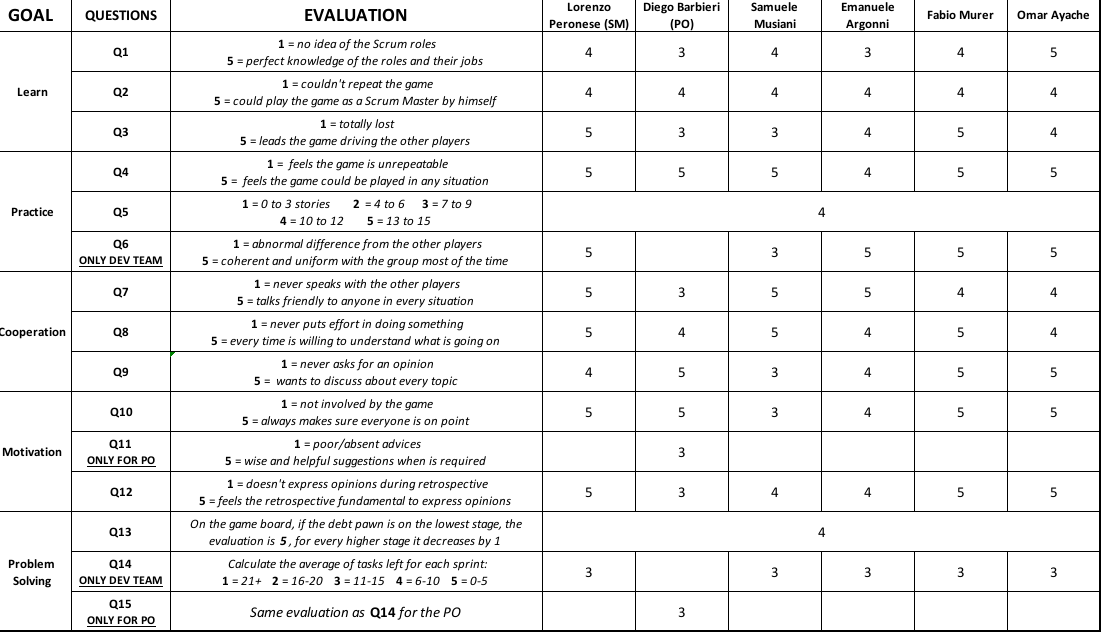
\includegraphics[width=1\textwidth]{report-scrumble}
    \caption{Tabella di autovalutazione del gioco \textit{Scrumble}}
    \label{fig:scrumble}
\end{figure}


\subsection{Gitinspector}

Le statistiche fornite dallo stakeholder Missiroli, generate tramite Gitinspector, non risultano essere accurate (il numero di commit 
segnalato da Gitinspector è di molto inferiore al numero reale). Non siamo riusciti a determinare con certezza se il problema risieda nel nostro 
repository o nel software stesso. Tuttavia, dopo aver effettuato ulteriori analisi indipendenti utilizzando Gitinspector, abbiamo riscontrato 
gli stessi risultati non corretti. Per completezza, i dati originali sono disponibili su 
\href{https://gitlab.vezgammon.it/diego/vezgammon/-/tree/main/doc/feedback_stakeholders}{\texttt{GitLab}}.

In questo report, vengono confivise invece le statistiche del repository ottenute tramite 
\href{https://github.com/git-quick-stats/git-quick-stats}{\texttt{git-quick-stats}}, un altro strumento di analisi. 

Si segnala che i dati riportati non includono la stesura di questo documento.

\begin{figure}[H] 
    \centering 
    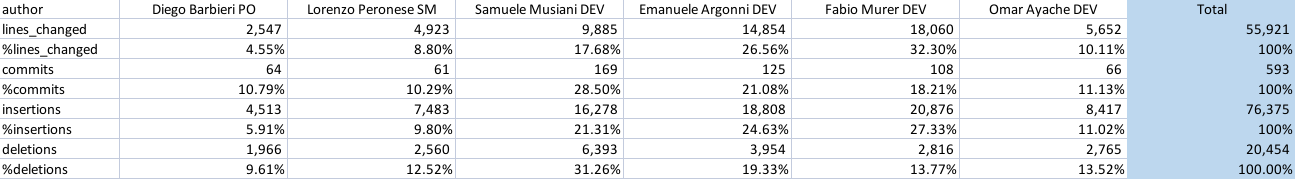
\includegraphics[width=\textwidth]{report-stats_raw} 
    \caption{Dati grezzi ricavati da git-quick-stats} 
    \label{fig:stats_raw} 
\end{figure}

\begin{figure}[H] 
    \centering 
    \begin{minipage}[t]{0.44\textwidth} 
        \centering 
        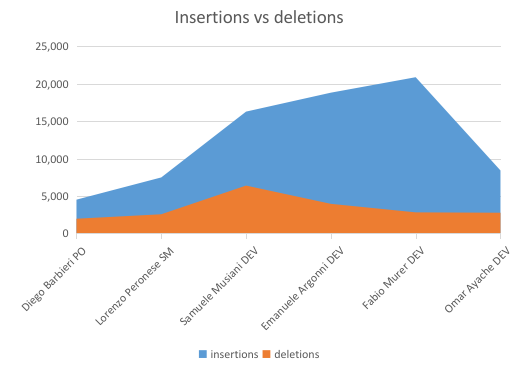
\includegraphics[width=\textwidth]{report-stats_insdel} 
        \caption{Rapporto tra linee inserite ed eliminate, le righe persistenti complessive sono oltre 55 mila} 
        \label{fig:stats_insdel} 
    \end{minipage} 
    \hfill 
    \begin{minipage}[t]{0.51\textwidth} 
        \centering 
        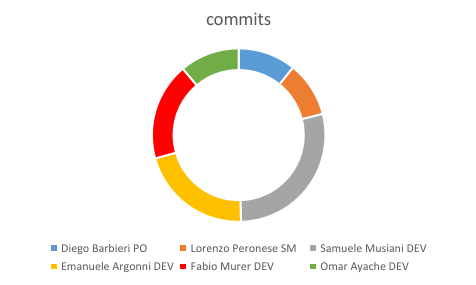
\includegraphics[width=\textwidth]{report-stats_commits} 
        \caption{Numero di commit nel repository, per un totale di 593 e una media di circa 15 al giorno} 
        \label{fig:stats_commits} 
    \end{minipage}
\end{figure}

\subsection{Monitoraggio delle ore}
Per il monitoraggio delle ore spese nel progetto non abbiamo utilizzato software di logging. Questa scelta è stata motivata dalla diversità di 
IDE utilizzati dai membri del team, che ha reso difficile individuare uno strumento compatibile per tutti. Inoltre, abbiamo provato inizialmente 
a utilizzare un timer per tracciare le ore, ma ci siamo resi conto che, non essendo un lavoro a tempo pieno, era comune dedicarsi ad altre 
attività durante le sessioni di scrittura del codice, questo rendeva il timer uno strumento poco adatto alla nostra situazione.

Abbiamo quindi optato per un approccio più semplice e flessibile, utilizzando un foglio Excel condiviso. Ogni membro del team ha segnato manualmente 
le ore effettivamente dedicate al progetto, garantendo una panoramica chiara e trasparente del tempo complessivamente investito. Di seguito quindi 
la tabella appena citata.

\begin{figure}[H]
    \centering
    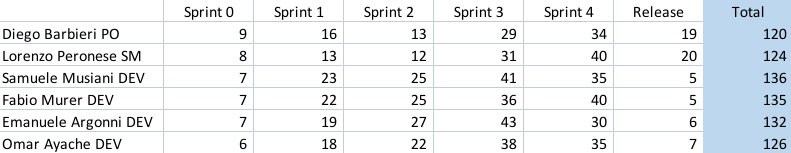
\includegraphics[width=1\textwidth]{report-logging_raw}
    \caption{Dati grezzi raccolti durante lo sviluppo}
    \label{fig:logging}
\end{figure}

\begin{figure}[H]
    \centering
    \begin{minipage}[t]{0.52\textwidth}
        \centering
        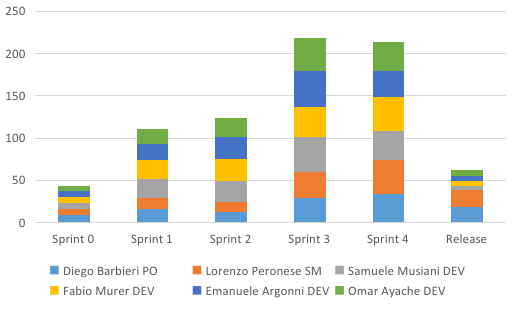
\includegraphics[width=\textwidth]{report-logging_sprints}
        \caption{Ore di lavoro per ogni sprint, il totale è 773 ore (32 interi giorni!)}
        \label{fig:logging-sprints}
    \end{minipage}
    \hfill
    \begin{minipage}[t]{0.47\textwidth}
        \centering
        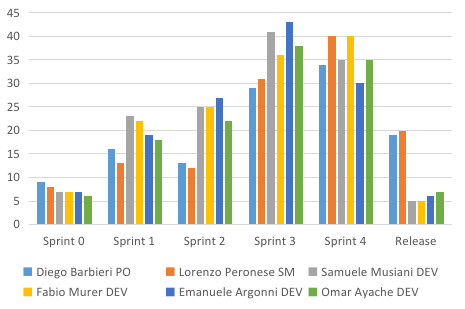
\includegraphics[width=\textwidth]{report-logging_full}
        \caption{Più nel dettaglio, ore di lavoro per membro del team per sprint}
        \label{fig:logging-full}
    \end{minipage}    
\end{figure}



\subsection{Strumenti di comunicazione} \label{sec:mm}
Per comunicare tra noi abbiamo deciso di usare MatterMost, una piattaforma di chat e condivisione interamente open-source. Come per gli altri 
servizi, anche MatterMost è stato self-hostato sotto il dominio \texttt{vezgammon.it} per avere un maggiore controllo sui dati. Questa scelta ha permesso 
di gestire in autonomia l'infrastruttura di comunicazione, evitando dipendenze da servizi esterni e assicurando la personalizzazione 
dell'ambiente in base alle necessità del progetto.

MatterMost è stato utilizzato per la comunicazione quotidiana, la condivisione di aggiornamenti e l'organizzazione degli incontri di persona, 
che si sono svolti con frequenza. Gli incontri hanno avuto luogo presso il laboratorio del gruppo ADMstaff, situato nel seminterrato del 
Dipartimento di Informatica, in Mura Anteo Zamboni 7.

Il laboratorio è diventato il punto di riferimento per il team, che vi si è riunito interi pomeriggi per \textit{Daily Scrum}, sessioni di \textit{pair programming} 
e discussioni sull'avanzamento generale del progetto. Questa modalità di lavoro ha favorito una collaborazione continua e diretta, contribuendo 
significativamente alla coesione del gruppo e al progresso del progetto.

Come strumento di comunicazione secondario è stato usato Telegram per comunicazioni meno "ufficiali" e sopratutto per ricevere notifiche relative 
allo stato dei vari servizi tramite \textit{Status} (vedi \ref{sec:status}).

\subsection{Utilizzo di Large Language Models}

Abbiamo integrato strategicamente diversi modelli di intelligenza artificiale generativa nello sviluppo del progetto. Nello specifico, abbiamo 
impiegato GitHub Copilot per l'autocompletamento del codice ripetitivo direttamente nell'IDE, Claude per la risoluzione di problematiche tecniche 
specifiche e ChatGPT per la stesura della documentazione.

L'approccio all'utilizzo di questi strumenti è stato mirato: per ogni problema, abbiamo scelto di impiegare l'AI o come supporto iniziale 
nell'esplorazione delle possibili soluzioni o come strumento per risolvere un particolare problema o perfezionare un'implementazione già esistente, 
evitando la sovrapposizione dei due metodi.

Nonostante questi strumenti abbiano contribuito a incrementare la produttività generale, il loro impiego ha richiesto particolare attenzione: le 
"allucinazioni" e gli errori nel codice generato hanno reso necessaria un'attenta verifica delle risposte e in diverse occasioni il tempo dedicato 
al debugging del codice generato ha superato il risparmio di tempo ottenuto nella sua scrittura.

Con l'esperienza, siamo giunti a un equilibrio efficace che ci ha permesso di sfruttare i punti di forza di questi potenti strumenti mantenendo al 
contempo un controllo adeguato per cercare di arginarne i lati negativi.

\subsubsection{Esempi di Prompt Utilizzati}

Di seguito sono riportati alcuni esempi a titolo esemplificativo dei prompt utilizzati, organizzati per categoria: \\ \\
\begin{tabular}{>{\columncolor{blue!30}}p{0.0001\textwidth} p{1\textwidth}}
    & - Fix this vue component error: \texttt{\{...\}} \\
    & - How do I refactor the code to make it work with tailwind themes? \texttt{\{...\}}\\
\end{tabular}
\begin{tabular}{>{\columncolor{green!30}}p{0.0001\textwidth} p{1\textwidth}}
    & - Given these SQL tables: \texttt{\{...\}} Make a SQL query to return the table \texttt{game} with usernames instead of \texttt{p1\_id}, \texttt{p2\_id}. \\
    & - PostgreSQL returns error: \texttt{syntax error at or near "FROM"} for the following query: \texttt{\{...\}} \\
\end{tabular}
\begin{tabular}{>{\columncolor{red!30}}p{0.0001\textwidth} p{1\textwidth}}
    & - Reformulate this user story: \texttt{\{...\}} Make it detailed enough for developers but not too technical for the client. \\
    & - This user story is too challenging: \texttt{\{...\}} Break it down into 3/4 smaller and more manageable user stories. \\
\end{tabular}
\begin{tabular}{>{\columncolor{orange!30}}p{0.0001\textwidth} p{1\textwidth}}
    & - How can I make this retrospective more objective and data-based? \texttt{\{...\}} \\
    & - How can I make this documentation more concise while maintaining all essential information? \texttt{\{...\}} \\
\end{tabular}

\subsection{SonarQube} \label{sec:sq}

\begin{figure}[H]
    \centering
    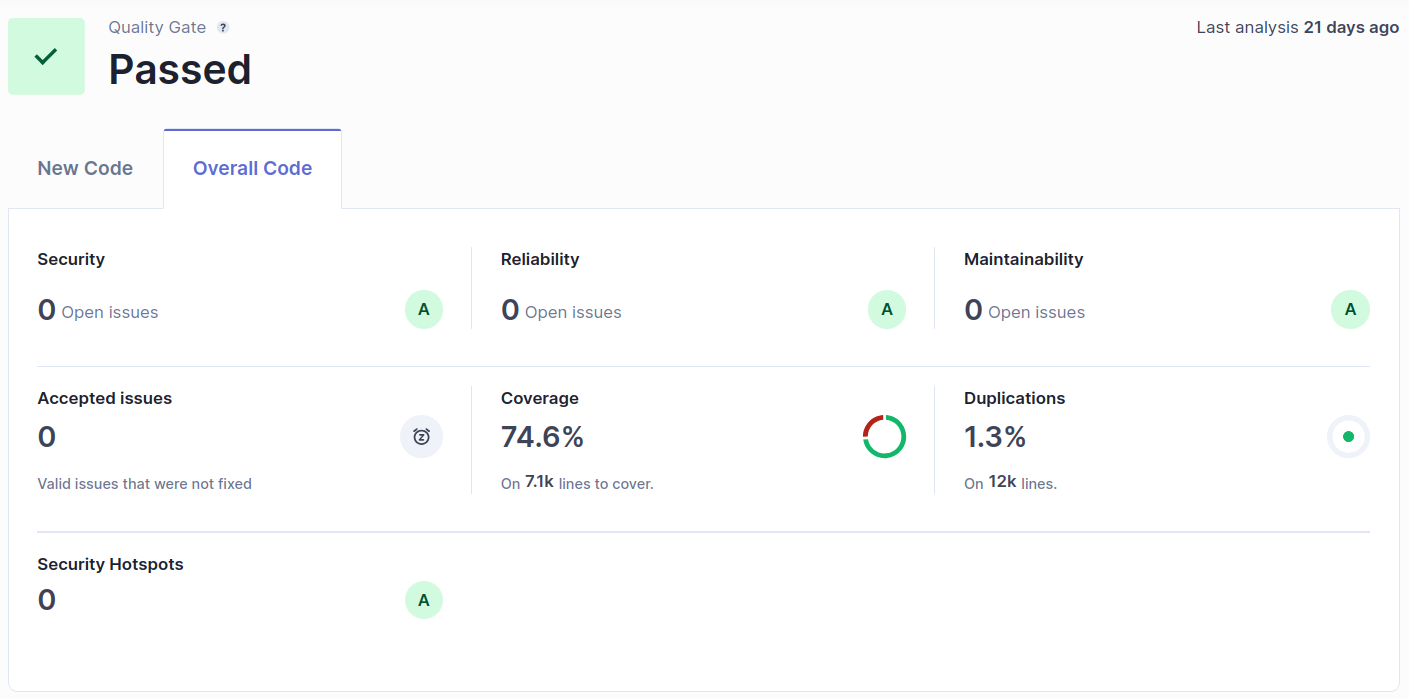
\includegraphics[width=1\textwidth]{report-sq_overview}
    \caption{Vista generale di SonarQube, che mostra un riepilogo delle metriche del progetto, tra cui copertura del codice, vulnerabilità, codice duplicato 
    e molto altro. \\
    L'obiettivo di una copertura del 50\% è stato abbondantemente superato; tuttavia le aree di codice meno coperte dai test riguardano principalmente le API 
    e le parti che fanno uso dei web socket, in quanto più difficili da testare.}
    \label{fig:sq_overview}
\end{figure}

\begin{figure}[H]
    \centering
    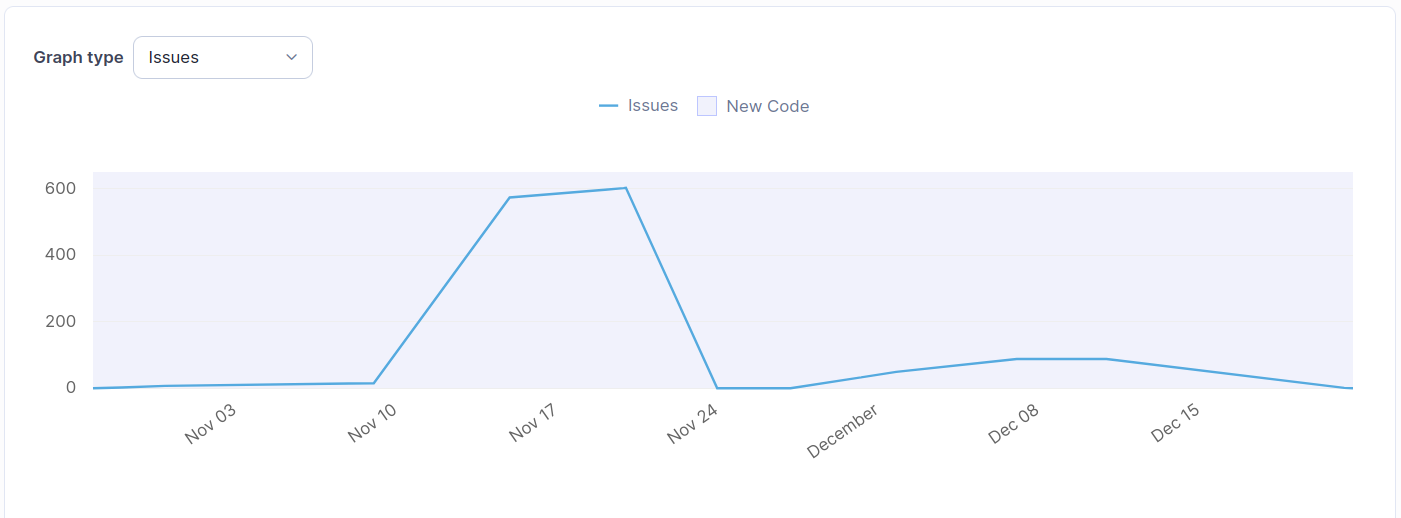
\includegraphics[width=1\textwidth]{report-sq_issues}
    \caption{Grafico delle issue rilevate nel tempo: il picco registrato intorno al 15 novembre è legato all'inclusione di due file HTML di GitInspector simili, 
    che ha portato SonarQube a rilevare numerosi problemi di duplicazione. Dopo aver individuato la causa, abbiamo escluso quei file dall'analisi, riportando 
    i valori alla normalità. Durante il resto dello sviluppo, il numero delle issue è stato mantenuto sotto controllo, risolvendo i problemi a intervalli regolari.}
    \label{fig:sq_issues}
\end{figure}


\section{Processo Scrum}

\subsection{Definition of Done}
Durante lo sprint 0 il \textit{Product Owner} ha definito i requisiti per dichiarare una user story come conclusa;
questi requisiti sono stati accettati dai developers e sono rimasti invariati durante tutta la durata dello sviluppo.

Vengono quindi riportati di seguito:

\subsubsection{Requisiti della Code Base}
\begin{itemize}
    \item Qualità del Codice
    \begin{itemize}
        \item Tutto il codice deve seguire le convenzioni di denominazione in camelCase.
        \item Ogni modulo deve avere e superare i propri test unitari (e mock, se sviluppato con TDD).
        \item Nessun codice critico o errori gravi rilevati dagli strumenti di analisi statica (es. SonarQube).
        \item Per le principali pagine del front-end, la funzionalità di base deve essere testata tramite test front-end.
    \end{itemize}

    \item Documentazione
    \begin{itemize}
        \item Tutte le API devono fornire un'anteprima con Swagger e includere test specifici per le API.
        \item README principale aggiornato con le funzionalità più recenti.
    \end{itemize}

    \item Merge Request
    \begin{itemize}
        \item Ogni merge request (MR) deve essere approvata dallo Scrum Master (SM) o dal Product Owner (PO).
        \item La MR deve superare tutti i test nella pipeline di testing di Jenkins.
    \end{itemize}

    \item Interfaccia Utente
    \begin{itemize}
        \item Soddisfa gli standard WCAG 2.1 AA: compatibile con tutti i browser moderni.
        \item Responsiva su laptop, tablet e smartphone (solo visualizzazione orizzontale).
    \end{itemize}

    \item Prestazioni
    \begin{itemize}
        \item L'app mantiene prestazioni accettabili (tempo di caricamento inferiore a 2 secondi per l'interfaccia principale del gioco).
    \end{itemize}
\end{itemize}

\subsubsection{Requisiti di Deployment}
\begin{itemize}
    \item Compatibilità
    \begin{itemize}
        \item L'applicazione funziona correttamente negli ambienti di sviluppo e produzione.
        \item L'applicazione deve richiedere un file di configurazione, facile da configurare e compatibile con l'architettura di deployment.
    \end{itemize}

    \item Build e Rilascio
    \begin{itemize}
        \item L'applicazione può essere compilata senza errori o avvisi.
        \item L'app è configurata per l'integrazione e il deployment continui, con test automatizzati per ogni merge.
    \end{itemize}

    \item Monitoraggio e Logging
    \begin{itemize}
        \item Sono attivi il monitoraggio degli errori in tempo reale e il logging front-end e back-end
        \item I log catturano eventi critici come l'inizio delle partite, le disconnessioni e gli errori dell'utente.
    \end{itemize}
\end{itemize}

\subsection{Definition of Ready}
Anche in questo caso, il documento \textit{Definition of Ready} è stato redatto dal \textit{Product Owner} all'inizio
dello sviluppo, accettato dal resto del team e durante gli sprint è rimasto pressocchè invariato.

Di seguito i requisiti che ogni user story deve avere per essere considerata \textit{ready}:

\begin{itemize}
    \item Il PBI è scritto in modo chiaro e conciso.
    \item Sono stati definiti criteri di accettazione testabili.
    \item Sono state identificate e risolte tutte le dipendenze.
    \item Tutti gli stakeholder hanno approvato il PBI.
    \item Le caratteristiche relative alla UI sono state discusse con il PO.
    \item Sono presenti requisiti tecnici (es. database, API).
    \item La documentazione preliminare (design, flussi di gioco) è completa.
    \item È stata fatta una stima delle ore di lavoro.
    \item Sono stati definiti i requisiti di accessibilità e usabilità.
    \item È stato convalidato con un piccolo gruppo di utenti (se necessario).
\end{itemize}

\subsection{Sprint 0}
Oltre alle attività di teambuilding (vedi \ref{sec:teambuilding}), i membri del gruppo hanno iniziato in questa fase a studiare
il funzionamento e la documentazione dei software scelti per lo sviluppo.

\subsection{Sprint 1}

\subsubsection{Goal}
Come si può vedere dallo snapshot di Taiga, lo sprint goal era piuttosto ambizioso e prevedeva 3 principali obiettivi:
\begin{itemize}
    \item creazione e gestione degli account;
    \item accesso a una partita;
    \item visualizzazione dei progressi di gioco.
\end{itemize}

\subsubsection{Backlog}
\begin{figure}[H]
    \centering
    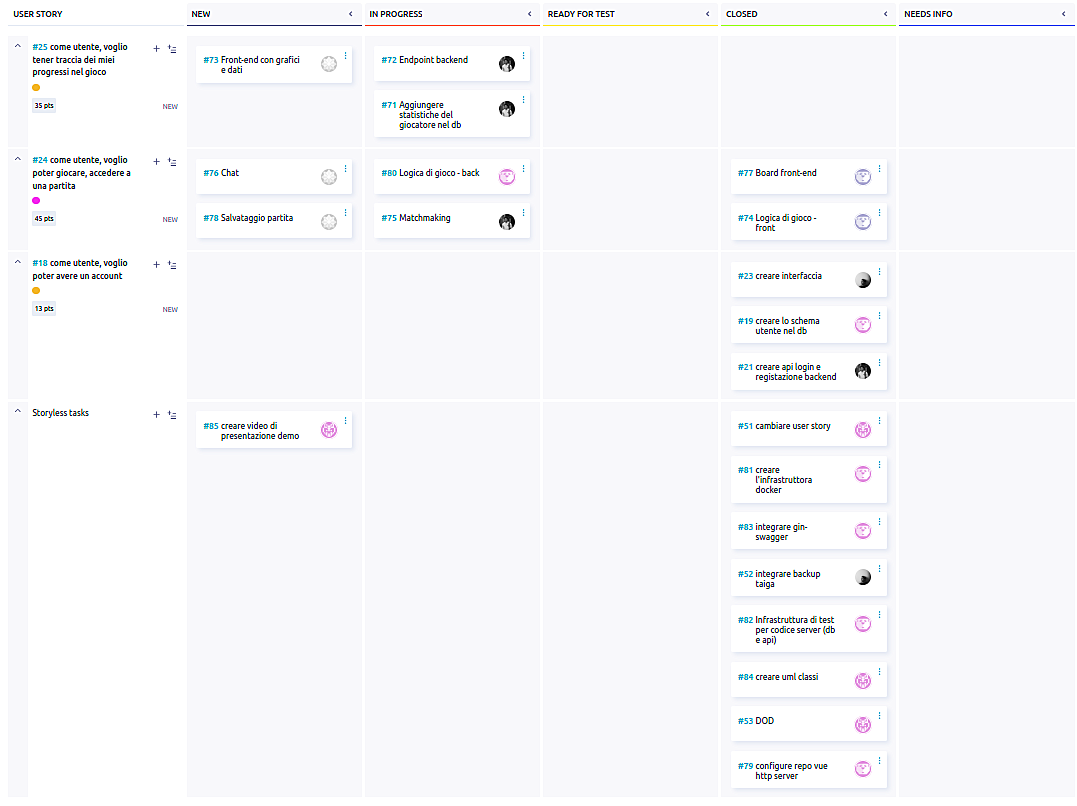
\includegraphics[width=1\textwidth]{backlog1}
    \caption{Backlog del primo sprint}
    \label{fig:backlog-s1}
\end{figure}

\subsubsection{Incremento}
Alla fine dello sprint, è stata completata con successo la user story che riguarda creazione e gestione dell'account 
(con autenticazione) ed era inoltre possibile giocare una partita locale molto semplice, tuttavia l'implementazione delle 
altre funzionalità chiave ha incontrato significative difficoltà:
\begin{itemize}
    \item sottostima del carico di lavoro;
    \item inefficace assegnazione delle user stories, troppo impegnative e generiche;
    \item complessità di integrazione con le nuove tecnologie;
    \item rallentamenti causati dal self-hosting dell'intero ambiente.
\end{itemize}

Un fattore critico è stato l'utilizzo di \texttt{Bgweb-api} per permettere di validare le mosse e giocare contro dei bot, 
che ha introdotto vincoli architetturali nella rappresentazione delle classi, in particolare le proprietà della partita. 
Questa scelta ha generato dipendenze che hanno rallentato lo sviluppo del backend anche durante gli sprint successivi.

\subsubsection{Esempio di test fatti}

\textbf{Creazione del profilo}
\begin{itemize}
    \item \underline{Obiettivo:} testare la registrazione di un utente
    \item \underline{Scenario:} un utente vuole creare un profilo utente registrandosi al sito
    \item \underline{Passaggi:}
    \begin{itemize}
        \item navigare alla home del sito
        \item Premere \textit{Sign up}
        \item Inserire tutti i campi correttamente
        \item Premere \textit{Register}
        \item effettuare il login
    \end{itemize}
    \item \underline{Risultato atteso:} l'utente deve essere creato correttamente e il login deve andare a buon fine
\end{itemize}

\subsubsection{Burndown}
\begin{figure}[H]
    \centering
    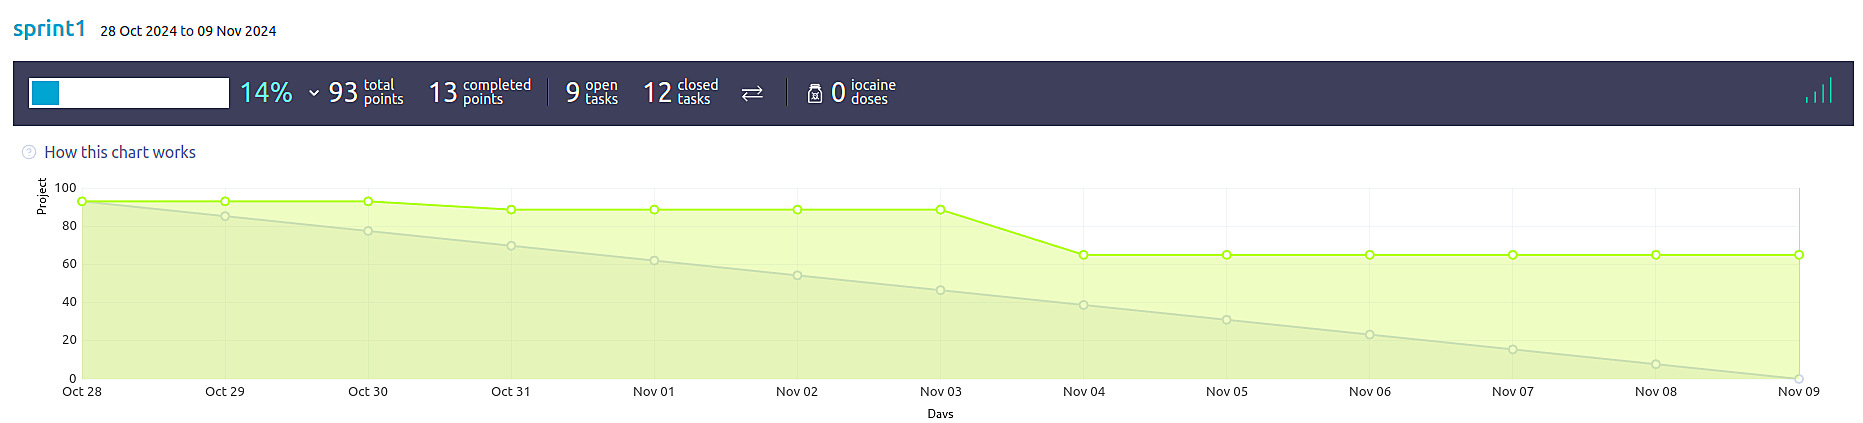
\includegraphics[width=1\textwidth]{burndown1}
    \caption{Burndown del primo sprint}
    \label{fig:burndown1}
\end{figure}

\subsubsection{Retrospettiva}

\begin{figure}[H]
    \centering
    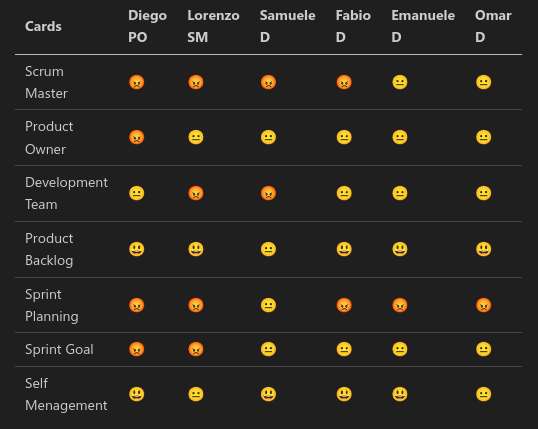
\includegraphics[width=1\textwidth]{retrospettiva1}
    \caption{Voti della retrospettiva del primo sprint}
    \label{fig:retrospettiva1}
\end{figure}

\textbf{Commenti personali}
\begin{itemize}
    \item \underline{Product Owner - Diego Barbieri}: \\
    Sotto-stima del carico di lavoro, specialmente riguardante la tecnologia per il back-end, che porterà ad un elevato debito tecnico del secondo sprint.
    Poco dialogo e male suddivisione dei compiti fra i developers. User story ben definite, task troppo vaghe. Suddivisione impari del carico di lavoro: 
    alcuni membri hanno lavorato più di altri.
    Veramente ottimo la gestione dell'ambiente di lavoro: server di deploy funzionante con un ottimo CI/CD.

    \item \underline{Scrum Master - Lorenzo Peronese}: \\
    Ottima gestione dell'ambiente di lavoro self-hostato, ma user stories troppo complesse e impegnative, soprattutto relative al back-end.
    Cattiva organizzazione della suddivisione delle task, anche a causa mia che ho dato scadenze poco precise
    e ho seguito troppo sommariamente lo sviluppo, senza aver capito a pieno lo scopo del mio ruolo.

    \item \underline{Developer - Samuele Musiani}: \\
    Sotto-stima del carico di lavoro, in particolare troppo per il backend e relativamente poco per il front-end.
    Il team per il front si è trovato bloccato da mancanza di features nel back.

    \item \underline{Developer - Fabio Murer}: \\
    Sotto-stima del carico di lavoro, sprint molto impegnativo a causa di user story troppo generali richiedenti molto lavoro.
    Continui problemi nel database mi hanno portato ad accumulare un ritardo nello sviluppo di features nella parte back-end.

    \item \underline{Developer - Emanuele Argonni}: \\
    Carico di lavoro sottostimato, abbiamo un elevato debito per il prossimo sprint. Era da pensare meglio la suddivisione delle user story considerati i 3 sprint. 
    PO e SM dovrebbero gestire meglio il team durante l'intero periodo dello sprint evitando di assegnare attività gli ultimi giorni prima della fine dello sprint.

    \item \underline{Developer - Omar Ayache}:\\
    Oltre ai commenti e riflessioni dei colleghi che condivido, vorrei che al prossimo sprint si prendesse in considerazione una specie di misura (i.e. i giorni 
    di lavoro o le ore) una misura quantitativa che associ task/tempo di lavoro. Questo dovrebbe comprendere anche la "tassa" della nuova tecnologia utilizzata, 
    per esempio il capire come funziona la gestione del db con pSQL (oppure i possibili problemi che possono nascere).
    I vantaggi dovrebbero essere che in questo modo riusciamo a valutare meglio sia il carico di lavoro ma anche il peso (punti) da assegnare ad ogni US.
\end{itemize} 

\noindent
\textbf{Prolematiche comuni e proposte per risolverle}

    Durante questo sprint, il carico di lavoro front-end è stato significativamente inferiore rispetto a quello back-end,
    causando tempi di inattività per gli sviluppatori front-end in attesa del completamento delle componenti server.
    Per ottimizzare gli sprint futuri, sarà fondamentale:
    \begin{itemize}

        \item bilanciare meglio la distribuzione delle attività tra front-end e back-end;
        \item garantire un flusso di sviluppo continuo e efficiente.

    \end{itemize}
    Il sovraccarico di user stories assegnate a questo sprint ha generato un debito tecnico considerevole che dovrà essere gestito
    nello sprint successivo. Di conseguenza, le attività inizialmente pianificate dovranno essere riprogrammate.
    Product Owner e Scrum Master si incontreranno lunedì per valutare strategie che evitino l'aggiunta di uno sprint
    supplementare rispetto alla pianificazione iniziale.
    Qualora l'estensione risultasse inevitabile, si procederà con una nuova distribuzione delle user stories.

\subsection{Sprint 2}

\subsubsection{Goal}
Lo sprint goal prevedeva lo sviluppo di \textit{core features} del gioco:
\begin{itemize}
    \item implementazione di un'interfaccia grafica strutturata;
    \item sviluppo di modalità di gioco locali (giocatore vs giocatore e giocatore vs bot) e online;
    \item personalizzazione dei temi grafici;
    \item implementazione del sistema di tracciamento dei progressi di gioco.
\end{itemize}

\subsubsection{Backlog}
\begin{figure}[H]
    \centering
    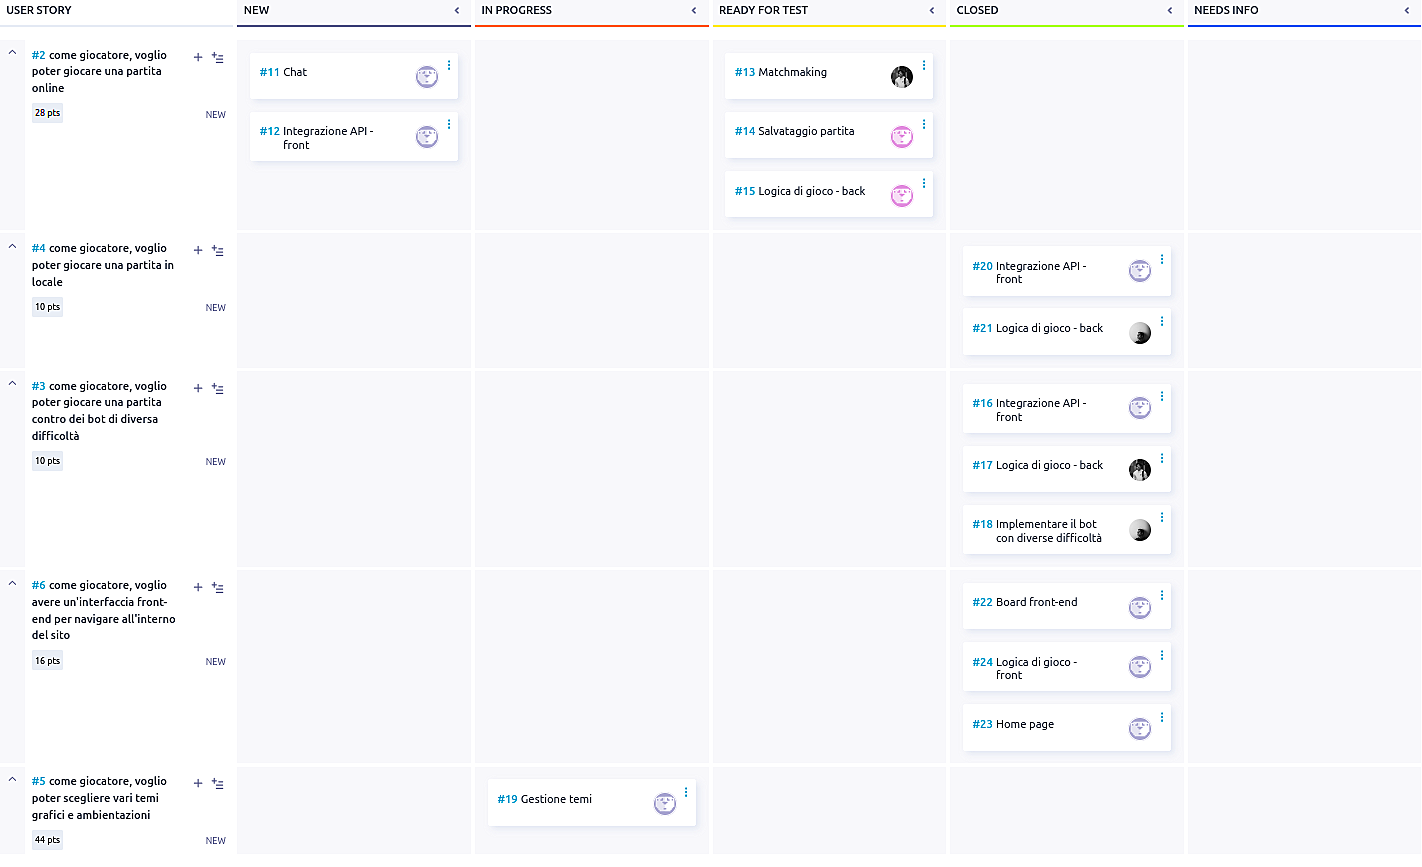
\includegraphics[width=1\textwidth]{backlog2_1}
    \caption{Backlog del secondo sprint - parte 1}
    \label{fig:backlog2_1}
\end{figure}

\begin{figure}[H]
    \centering
    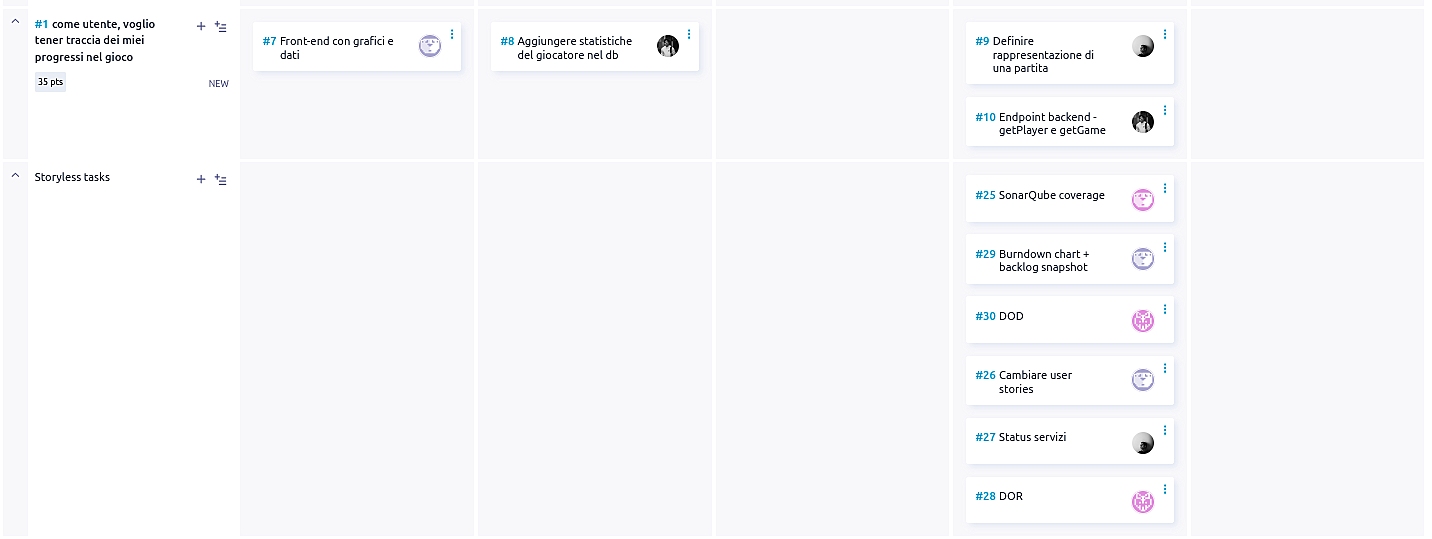
\includegraphics[width=1\textwidth]{backlog2_2}
    \caption{Backlog del secondo sprint - parte 2}
    \label{fig:backlog2}
\end{figure}

Purtroppo l'immagine originale era molto sfocata, quindi ho riprodotto il progetto di Taiga per fare questi screenshots.

Per questo motivo i numeri sulle user stories e sui task non coincidono con quelli delle altre immagini.

\subsubsection{Incremento}
Queste sono le user stories completate:
\begin{itemize}
    \item interfaccia front-end strutturata per la navigazione del sito;
    \item partita locale (su un unico schermo);
    \item partita contro bot di diversa difficoltà.
\end{itemize}
Le storie non completate, quindi il debito tecnico, sono state la gestione della partita online (sempre a causa del validatore
di mosse e della difficoltà ad interfacciarsi ad esso), l'implementazione di altri temi grafici e, ancora una volta, la dashboard
con i progressi di gioco.

\subsubsection{Esempio di test fatti}

\textbf{Giocare una partita in locale}
\begin{itemize}
    \item \underline{Obiettivo:} Verificare che si possa creare e giocare una partita in locale
    \item \underline{Scenario:} Un utente crea una partita in locale, si effettuano due turni e si chiude la partita abbandonando
    \item \underline{Passaggi:}
    \begin{itemize}
        \item un utente crea una partita in locale
        \item effettua il turno 1
        \item effettua il turno 2
        \item chiude la partita abbandonando
        \end{itemize}
    \item \underline{Risultato atteso:} la partita viene creata con lo stesso giocatore come giocatore 1 e 2, i due turni si possono giocare 
    dallo stesso giocatore, dopo l'abbandono la partita viene chiusa e lo stato viene messo a winp2
\end{itemize}

\subsubsection{Burndown}
\begin{figure}[H]
    \centering
    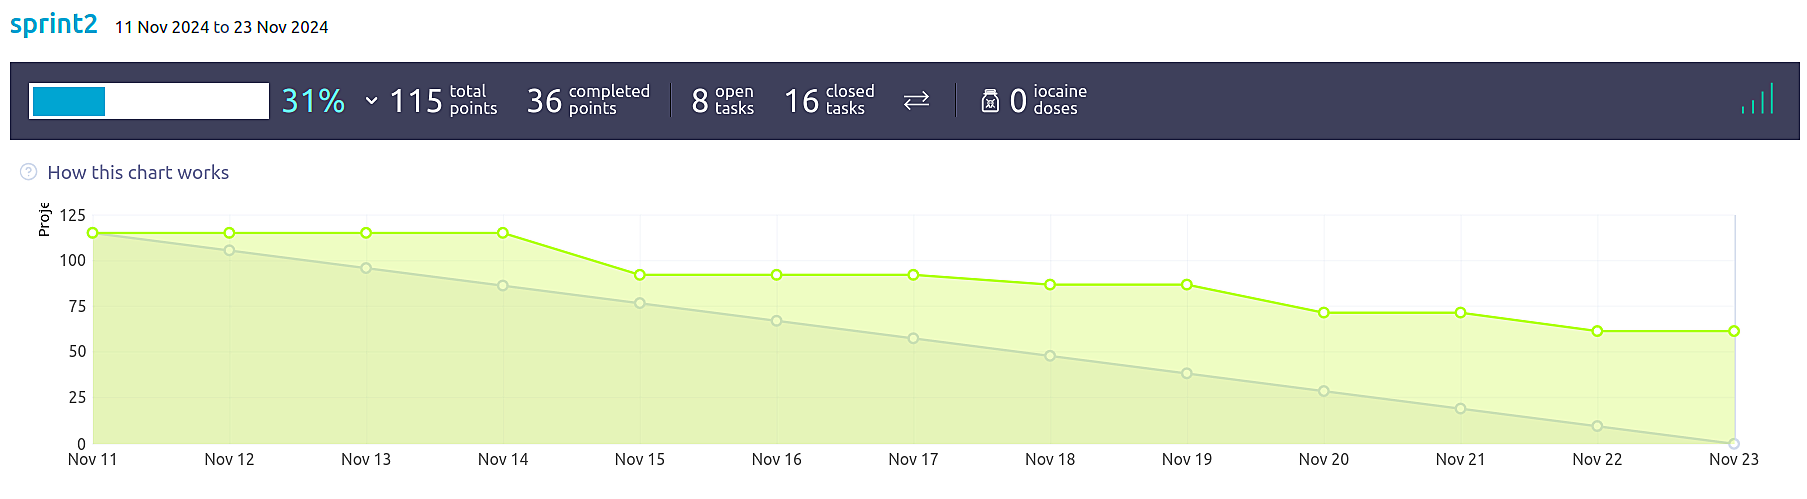
\includegraphics[width=1\textwidth]{burndown2}
    \caption{Burndown del secondo sprint}
    \label{fig:burndown2}
\end{figure}

\subsubsection{Retrospettiva}

\begin{figure}[H]
    \centering
    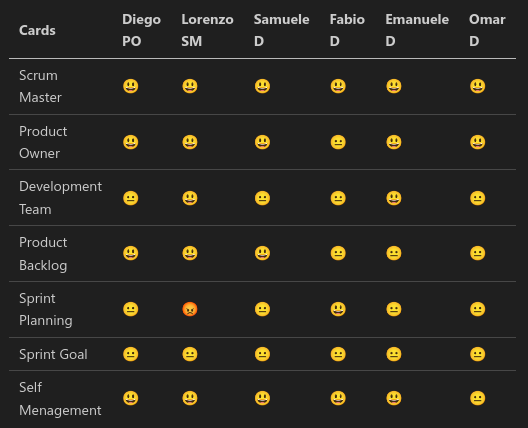
\includegraphics[width=1\textwidth]{retrospettiva2}
    \caption{Voti della retrospettiva del secondo sprint}
    \label{fig:retrospettiva2}
\end{figure}

\textbf{Commenti personali}
\begin{itemize}
    \item \underline{Product Owner - Diego Barbieri}: \\
    Nel complesso, penso che il team abbia lavorato al meglio delle proprie capacità. Sono stati parzialmente risolti i problemi di comunicazione
    e di suddivisione del carico di lavoro. Penso che sia necessaria maggiore attenzione agli standard da adottare per le API tra front e back-end.
    Questo puo' essere risolto con una maggiore attenzione agli schemi di progettazione e alla documentazione.
    Sono stato negativamente colpito dal fatto che durante l'ultima sprint review, alcuni membri del team non avessero ben chiaro il significato di DOD
    e della sua importanza. Lo stesso e' successo quando un developer ha mergiato direttamente sul main parte dello sviluppo ancora non pienamente completato.

    \item \underline{Scrum Master - Lorenzo Peronese}: \\
    Tutti hanno lavorato di più e meglio, con maggior comunicazione e aiuto reciproco.
    I daily scrum sono stati strutturati meglio e sono passati da una frequenza irregolare a una cadenza fissa ogni due giorni; sono stati un momento utile per
    tutti di confronto e discussione.
    Unica nota negativa è stata ancora una volta una cattiva pianificazione dello sprint: 3 user stories su 6 complessive non sono state
    completate a causa di una stima sbagliata a inizio sprint e molti problemi imprevisti emersi durante queste due settimane; è stato richiesto molto impegno 
    ai developers ma sono soddisfatto del modo in cui queste difficoltà sono state affrontate e superate.

    \item \underline{Developer - Samuele Musiani}: \\
    Problemi nel back-end, soprattutto riguardo le api per backgammon. Sotto-stima dei tempi per completare certe US. Buona la scelta di spostare
    un developer del frontend nel backend.

    \item \underline{Developer - Emanuele Argonni}: \\
    Purtroppo anche per questo sprint non siamo riusciti a portare a termine tutte la task,
    dato un incoveniente con le API del backend che non ritornavano tutte le mosse possibili
    Nella seconda settimana dello sprint grazie al pair-programming tra backend e frontend siamo riusciti a risolvere quasi tutti i problemi riscontrati,
    nonostante il tempo perso per il debugging.
    Buon lavoro dello scrum master che ha cercato di motivare i developer ed ha organizzato i daily scrum per permettere ai membri del team di confrontarsi
    
    \item \underline{Developer - Omar Ayache}:\\
    Sottostima del lavoro e problemi riguardo gestione del bot per le mosse, ottimo l'utilizzo della strategia pair-programming per i prossimi sprint.
    Miglior presa di coscienza generale del carico di lavoro.    
\end{itemize} 

\noindent
\textbf{Prolematiche comuni e proposte per risolverle}
Dall'analisi delle opinioni raccolte emerge un miglioramento generale delle prestazioni del team rispetto allo sprint precedente, sebbene persistano alcune criticità 
nella stima del carico di lavoro e nella comunicazione interna. Alla luce di queste considerazioni, proponiamo le seguenti azioni per il prossimo sprint:
\begin{itemize}
    \item effettuare piu' pair-programming per risolvere problemi di comunicazione. Questo permetterebbe di mettere in diretta relazione persone di diversi ruoli e 
    di far capire meglio il lavoro che si sta svolgendo;
    \item suddividere il carico di lavoro includendo anche PO e SM in attività di sviluppo, per massimizzare e parallelizzare il lavoro. Questo non sottraendo tempo 
    alle attività già previste dai loro ruoli.
\end{itemize}

\subsection{Sprint 3}

\subsubsection{Goal}
L'obiettivo di questo terzo sprint era dare un'importante accellerata allo sviluppo, pertanto il carico di lavoro è stato molto maggiore ma la situazione lo richiedeva.
Per agevolare la buona riuscita dello sprint sono stati adottati diversi principi Agili:
\begin{itemize}
    \item \textit{Scrum Master} e \textit{Product Owner} hanno dato una mano nella scrittura del codice, oltre a mantenere i loro ruoli abituali;
    \item i \textit{Daily Scrum} sono stati più frequenti e articolati per pianificare e gestire al meglio il tempo a disposizione;
    \item \textit{pair programming} tra sviluppatori front-end e back-end.
\end{itemize}
Le user stories previste per questo sprint riguardavano: 
\begin{itemize}
    \item dashboard con progressi di gioco;
    \item gestione di una partita online;
    \item replay e analisi delle partite giocate;
    \item gestione di nuovi temi;
    \item gestione di badge digitali al raggiungimento di determinati obiettivi;
    \item chat durante le partite;
    \item risorse di addestramento (tutorial e regole di gioco);
    \item condivisione dei progressi di gioco sui social.
\end{itemize}

\subsubsection{Backlog}
\begin{figure}[H]
    \centering
    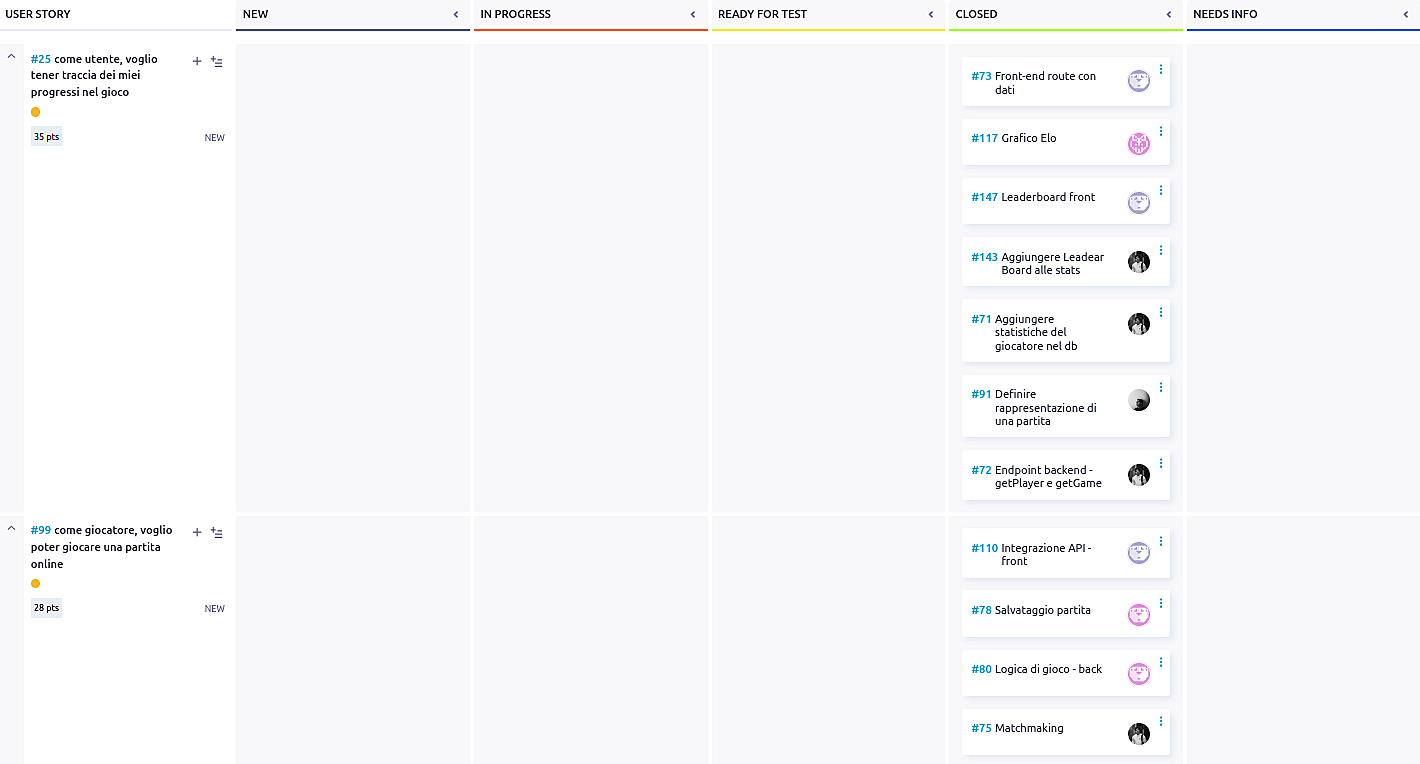
\includegraphics[width=1\textwidth]{backlog3_1}
    \caption{Backlog del terzo sprint - parte 1}
    \label{fig:backlog3_1}
\end{figure}

\begin{figure}[H]
    \centering
    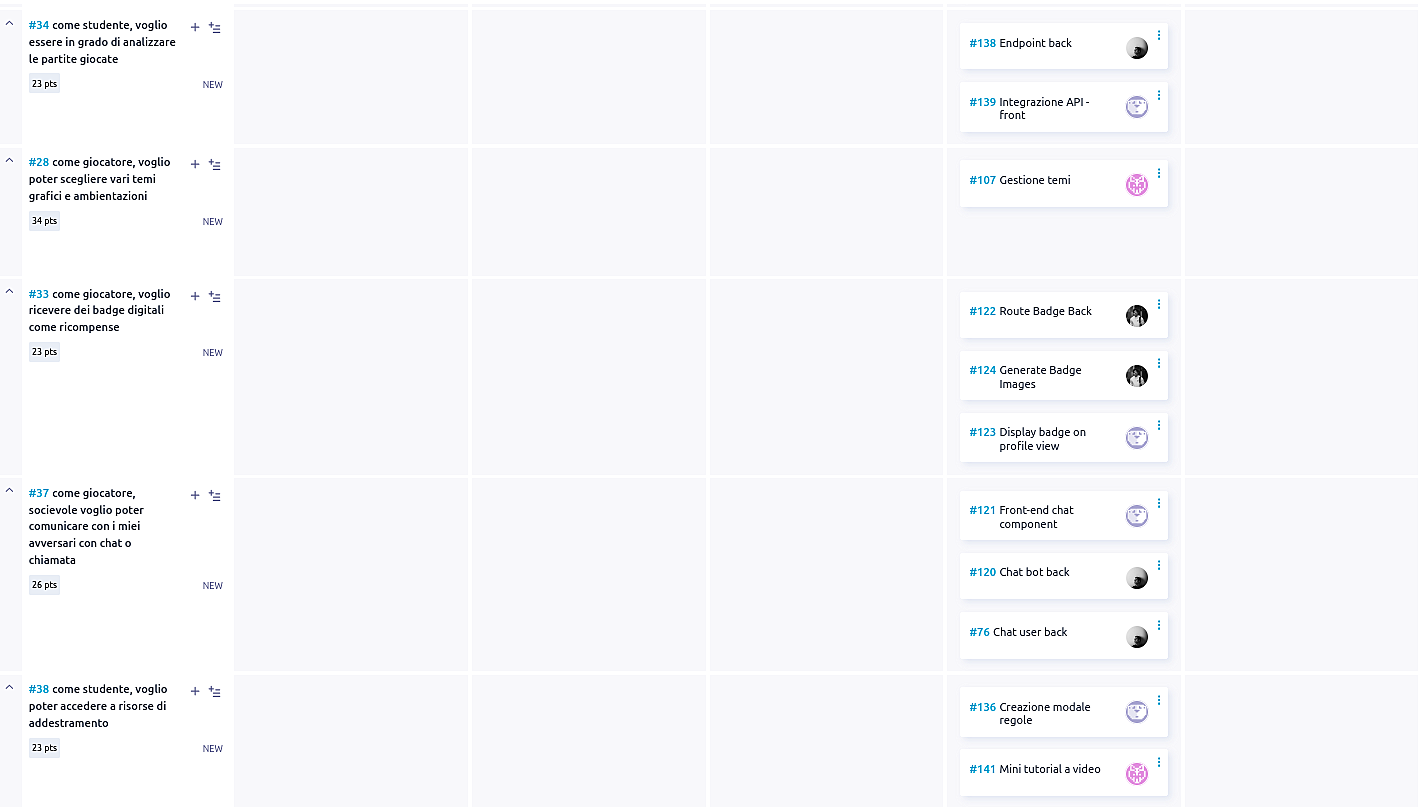
\includegraphics[width=1\textwidth]{backlog3_2}
    \caption{Backlog del terzo sprint - parte 2}
    \label{fig:backlog3_2}
\end{figure}

\begin{figure}[H]
    \centering
    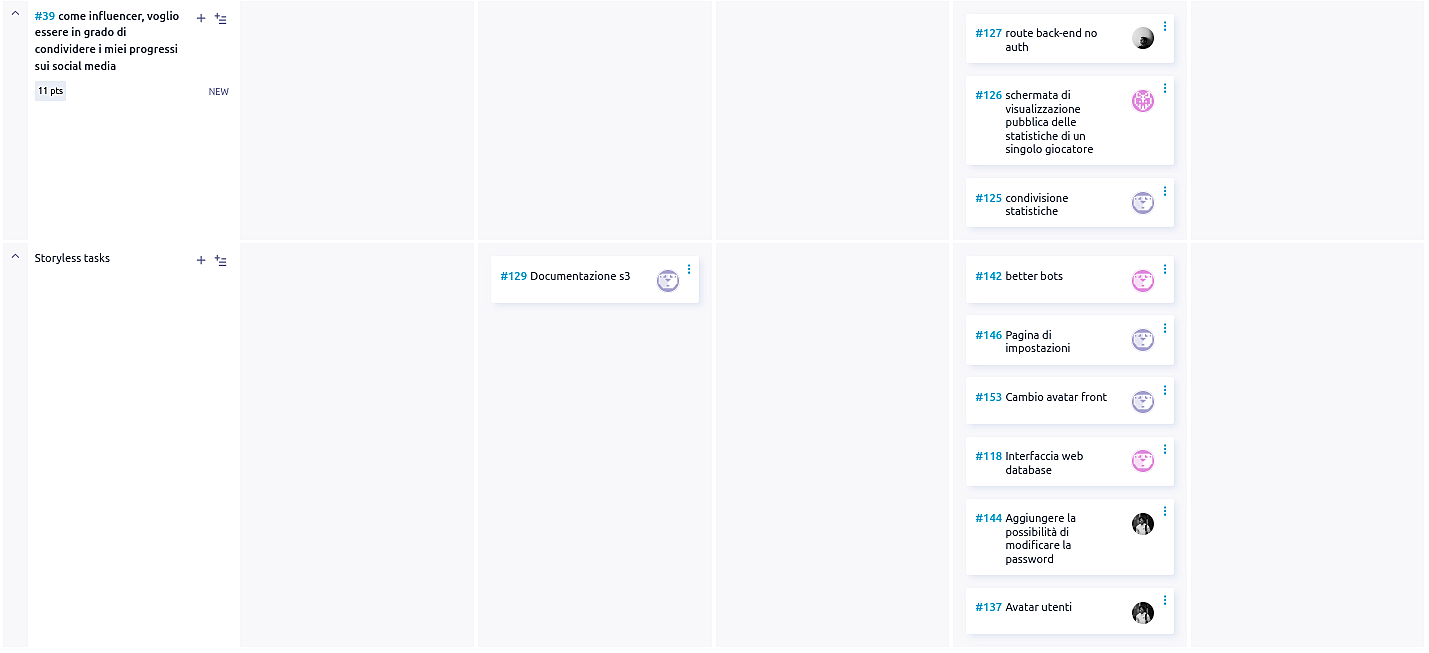
\includegraphics[width=1\textwidth]{backlog3_3}
    \caption{Backlog del terzo sprint - parte 3}
    \label{fig:backlog3_3}
\end{figure}

\subsubsection{Incremento}
Questo sprint ha richiesto un enorme sforzo da parte di tutti, è stato di gran lunga quello con più user stories ma ciò nonostante è stato il primo in cui 
tutte le user stories sono state completate con successo, senza debito tecnico.

\subsubsection{Esempio di test fatti}

\textbf{Generazione badge}
\begin{itemize}
    \item \underline{Obiettivo:} testare la creazione di generazione del badge prima vittoria
    \item \underline{Scenario:} un giocatore vince la prima partita
    \item \underline{Passaggi:}
    \begin{itemize}
    \item creare una partita
    \item vincere la partita
    \end{itemize}
    \item \underline{Risultato atteso:} il giocatore deve avere il badge \textit{first victory}
\end{itemize}

\subsubsection{Burndown}
\begin{figure}[H]
    \centering
    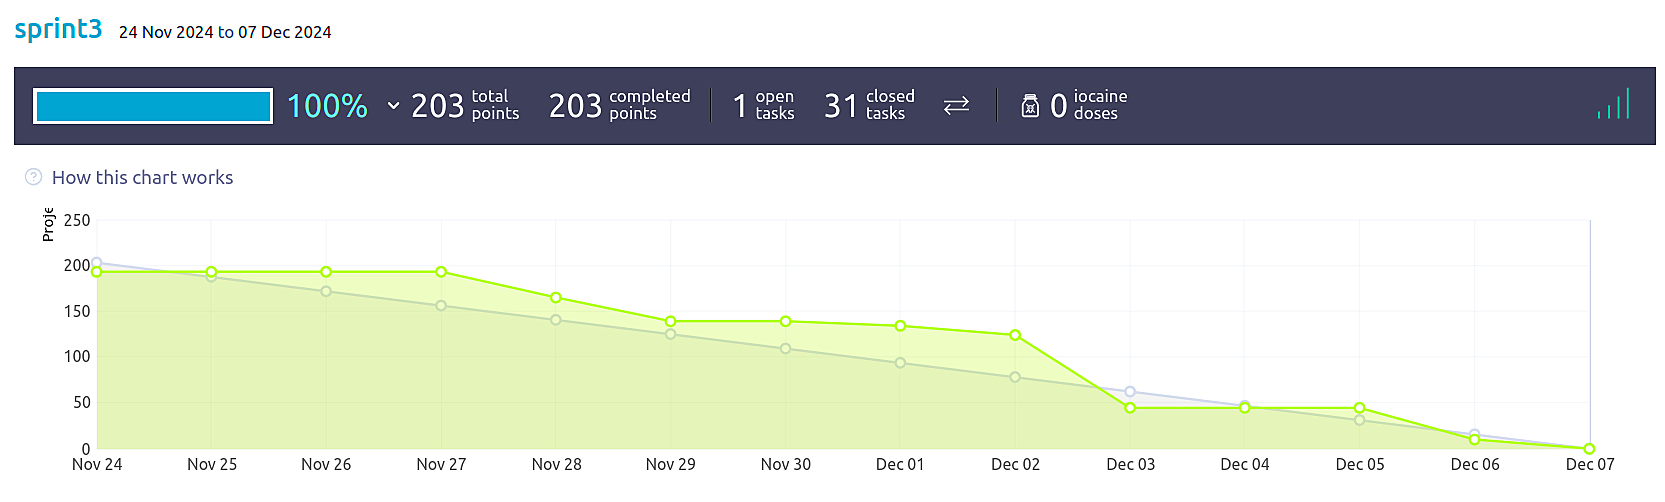
\includegraphics[width=1\textwidth]{burndown3}
    \caption{Burndown del terzo sprint}
    \label{fig:burndown3}
\end{figure}

\subsubsection{Retrospettiva}
\begin{figure}[H]
    \centering
    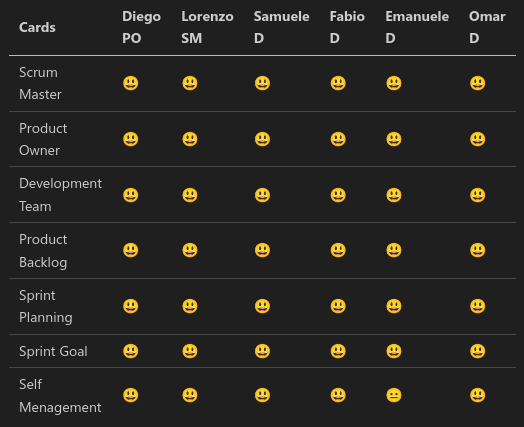
\includegraphics[width=1\textwidth]{retrospettiva3}
    \caption{Voti della retrospettiva del terzo sprint}
    \label{fig:retrospettiva3}
\end{figure}

\textbf{Commenti personali}
\begin{itemize}
    \item \underline{Product Owner - Diego Barbieri}: \\
    Ottimo sprint, in assoluto il migliore. Nonostante un primo momento di insicurezza generale sul superamento delle task, ci siamo trovato a meta' settimna con 
    tutte le us quasi completate: e' risultato necessario un "daily scrum on steroids" per decidere ulteriori us da terminare. Alla fine sono molto soddisfatto del 
    risultato ottenuto, il tutto grazie a un codice ben organizzato in componenti.
    \item \underline{Scrum Master - Lorenzo Peronese}: \\
    Sprint eccellente, con il completamento di tutte le user stories assegnate. Gli imprevisti sono stati pochi e ben gestiti, grazie a uno sviluppo costante 
    supportato dai tre daily scrum settimanali e da una comunicazione efficace, sia in chat che di persona in laboratorio. Il pair programming si è rivelato 
    un grande successo, consentendo di risolvere molte problematiche in modo rapido ed efficace.
    \item \underline{Developer - Samuele Musiani}: \\
    Sprint decisamente positivo sotto molteplici aspetti. Il gruppo ha dimostrato un'ottima cooperazione che ha portato al completamento di quasi tutte le US 
    con un anticipo notevole rispetto alle tempistiche preventivate. Il team ha inoltre dimostrato una completa padronanza degli strumenti utilizzati, potendo quindi 
    focalizzare le proprie risorse principalmente sulle attività di implementazione, ottimizzando così l'efficienza dell'intero processo di sviluppo. Questo sprint 
    testimonia la maturità del gruppo e pone solide basi per il proseguimento del progetto.
    \item \underline{Developer - Emanuele Argonni}: \\
    Sicuramente il migliore sprint fino ad ora, siamo riusciti a completare quasi tutte le task assegnate, nonostante avessimo un importante debito derivato 
    dagli sprint precedenti.
    Il team dei developer ha lavorato bene e si è dimostrato molto collaborativo. Il lavoro di squadra è stato fondamentale per il raggiungimento degli obiettivi.
    Il pair programming è stato molto utile per l'integrazione backend-frontend e per risolvere i problemi che si sono presentati durante lo sprint.
    Terminate le task assegnate, ci siamo dedicati al refactor del codice per migliorare la chiarezza e la manutenibilità del codice.
    \item \underline{Developer - Omar Ayache}:\\
    Sprint eccezionale, con obiettivi quasi completamente raggiunti. Diversi meeting scrum dinamici hanno permesso di ridefinire ulteriori attività. Il team ha dimostrato 
    una significativa crescita, padroneggiando con competenza gli strumenti e comprendendo la loro complessità di utilizzo. L'organizzazione del codice in componenti 
    ben strutturate ha contribuito al successo complessivo.    
\end{itemize} 

\subsection{Sprint 4}

\subsubsection{Goal}
Il goal di questo ultimo sprint è stato dedicato all'ultima \textit{core feature}, ovvero i tornei, sia con altri giocatori che con bot di diversa difficoltà.
Inoltre, in queste due settimane l'obiettivo era quello di rendere l'intera app responsive e usufruibile da cellulare e ricevere
notifiche in app, ad esempio alla ricezione di nuovi badge o durante la partecipazione a un torneo.

\subsubsection{Backlog}
\begin{figure}[H]
    \centering
    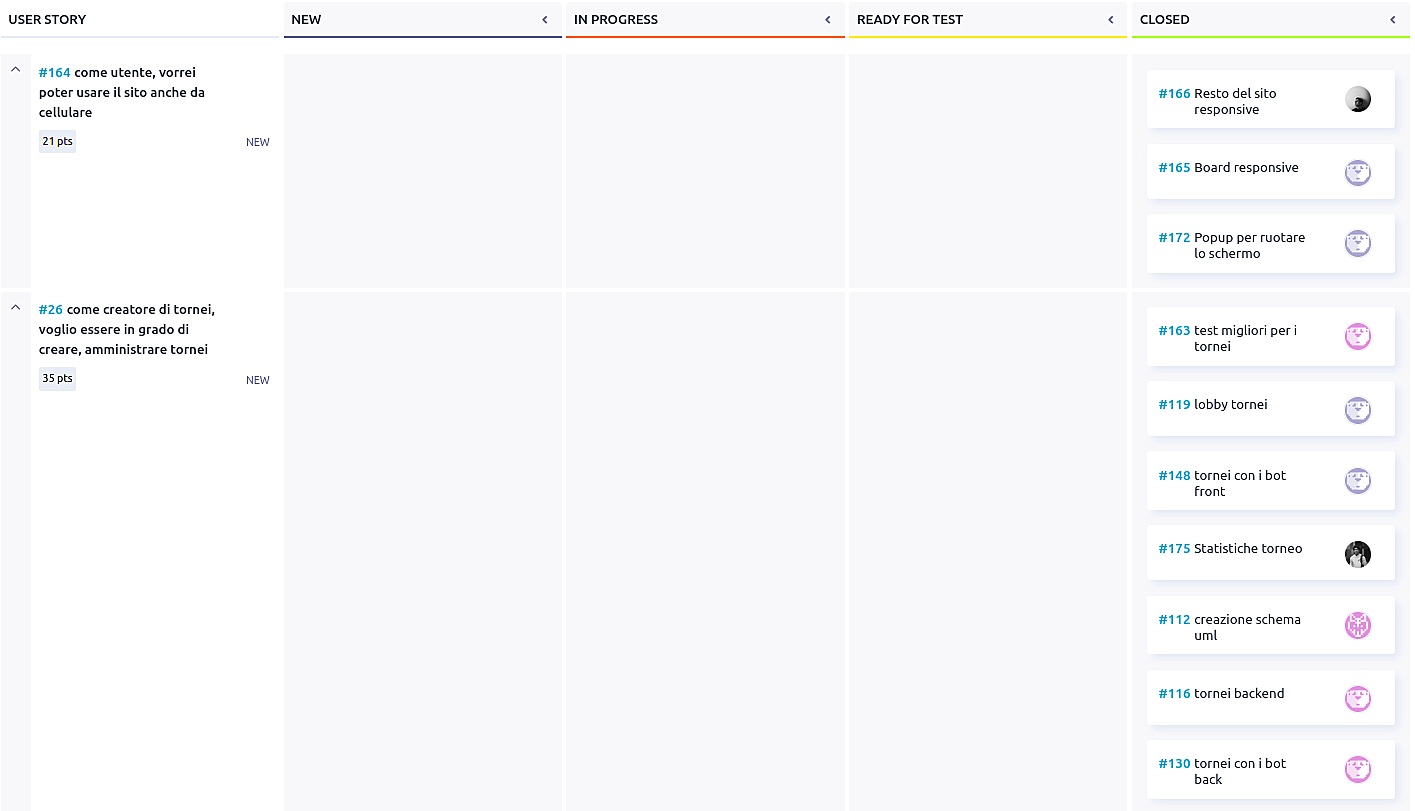
\includegraphics[width=1\textwidth]{backlog4_1}
    \caption{Backlog del quarto sprint - parte 1}
    \label{fig:backlog4_1}
\end{figure}

\begin{figure}[H]
    \centering
    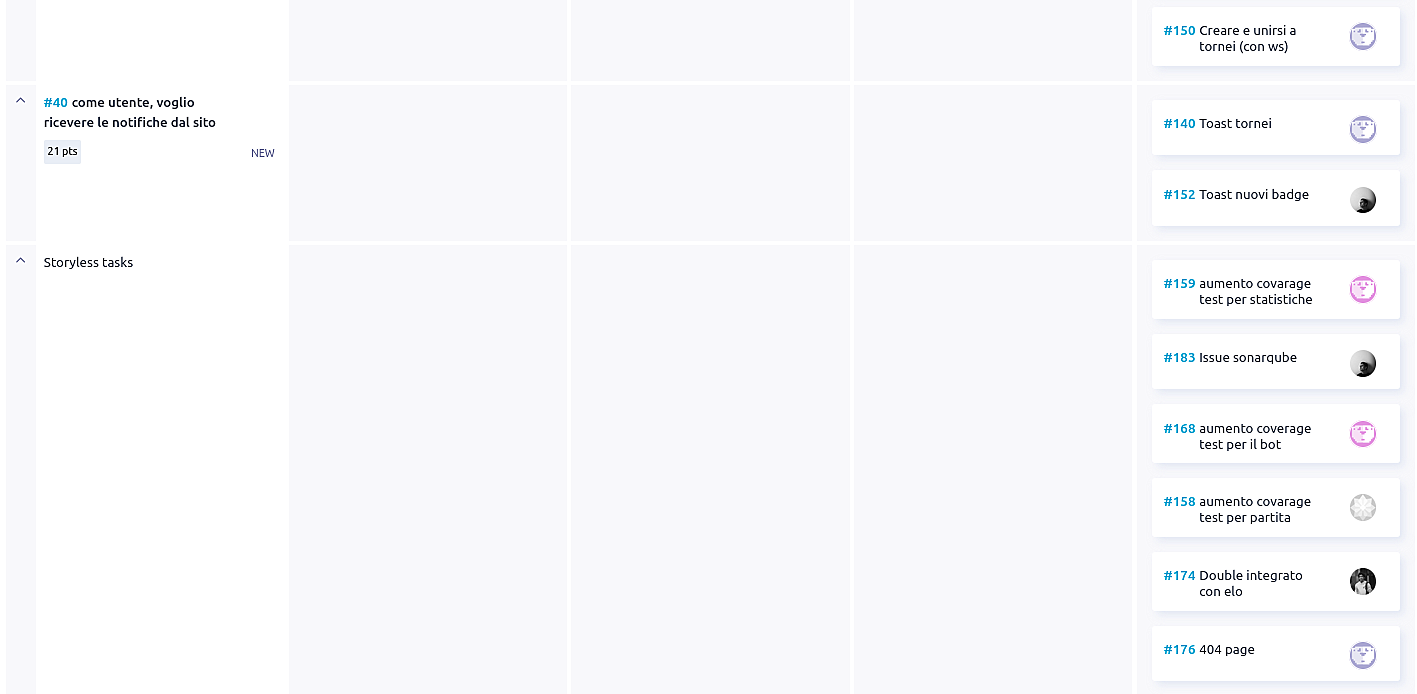
\includegraphics[width=1\textwidth]{backlog4_2}
    \caption{Backlog del quarto sprint - parte 2}
    \label{fig:backlog4_2}
\end{figure}

\subsubsection{Incremento}
Anche in questo sprint tutte le task sono state completate con successo, non scontato data la sovrapposizione con l'inizio della
sessione invernale d'esami. 

\subsubsection{Esempio di test fatti}

\textbf{Verificare che il torneo venga creato correttamente}
\begin{itemize}
    \item \underline{Obiettivo:} Verificare un utente possa creare un torneo e questo sia creato correttamente
    \item \underline{Scenario:} Un utente crea un torneo
    \item \underline{Passaggi:}
    \begin{itemize}
        \item navigare all'interfaccia di creazione tornei
        \item inserire il nome del torneo che si vuole creare
        \item creare un torneo utilizzando l'apposito bottone
    \end{itemize}
    \item \underline{Risultato atteso:} un nuovo torneo deve essere creato con i seguenti campi: l'utente che lo ha creato come owner, come unico utente l'owner 
    e come stato waiting
\end{itemize}

\subsubsection{Burndown}
\begin{figure}[H]
    \centering
    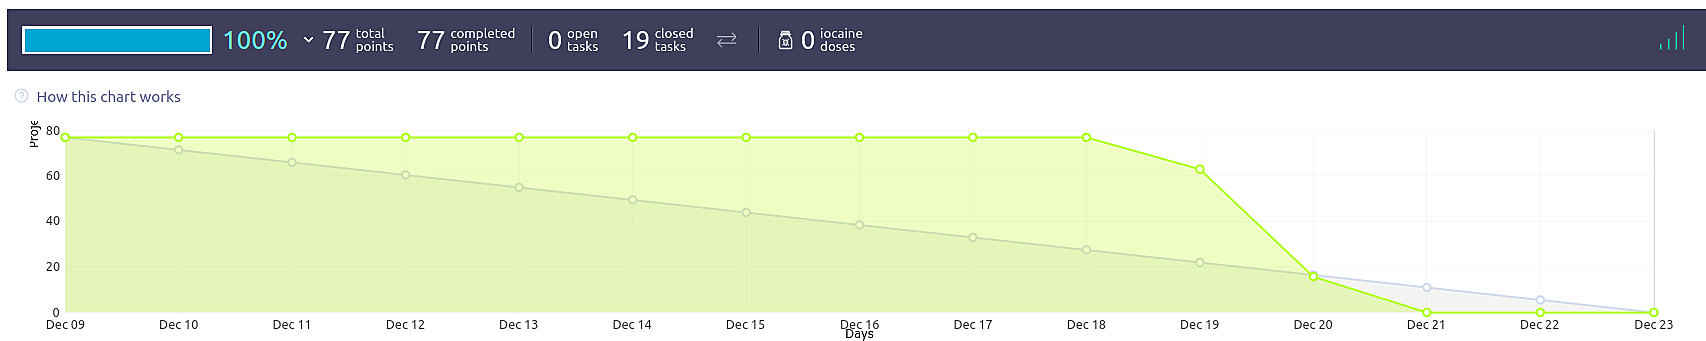
\includegraphics[width=1\textwidth]{burndown4}
    \caption{Burndown del quarto sprint}
    \label{fig:burndown4}
\end{figure}

\subsubsection{Retrospettiva}

\begin{figure}[H]
    \centering
    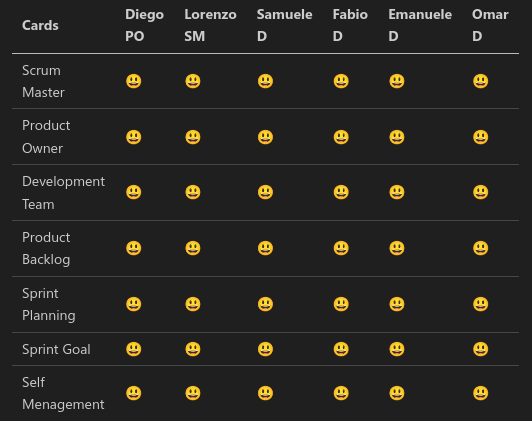
\includegraphics[width=1\textwidth]{retrospettiva4}
    \caption{Voti della retrospettiva del quarto sprint}
    \label{fig:retrospettiva4}
\end{figure}

\textbf{Commenti personali}
\begin{itemize}
    \item \underline{Product Owner - Diego Barbieri}: \\
    Sprint molto positivo, quasi quanto il precedente, ovviamente con un carico di lavoro minore. Simao riusciti a portare tutto al termine, 
    grazie ad un ottima organizzazione del team, maturata durante tutto questo viaggio.
    \item \underline{Scrum Master - Lorenzo Peronese}: \\
    Durante lo sprint tutti hanno lavorato bene e in sinergia, portando a termine tutte le user stories nei tempi previsti nonostante l'inizio degli esami. 
    Il pair programming tra frontend e backend e i daily scrums sono sono diventate abitudini Agili e si sono rivelate fondamentali per gestire 
    il doppio impegno studio-lavoro senza sacrificare la qualità del codice. Questo e il precedente sprint dimostrano il miglioramento 
    che c'è stato rispetto alle prime settimane, il team è riuscito a prendere il ritmo giusto e concludere il lavoro nel migliore dei modi.
    \item \underline{Developer - Samuele Musiani}: \\
    Sprint positivo, soprattutto a seguito della conclusione di tutte le US assegnate. Il team ha lavorato bene nonostante l'inzio degli esami universitari,
    portando a termine ogni compito nel tempo previsto. Si riconfermata la piena padronanza degli strumenti utilizzati e la capacità di coordinarsi per portare a termine
    tutte le task più complesse che richiedevano una collaboraione tra frontend e backend.
    \item \underline{Developer - Fabio Murer}: \\
    Sprint positivo, grazie ai daily scrum frequenti e il lavoro a stretto contatto tra backend e frontend questo sprint 
è risultato molto positivo permettendoci di risolvere velocemente le task e di risolvere un gran numero di bug.
    \item \underline{Developer - Emanuele Argonni}: \\
    Questo sprint, come il precedente, ha evidenziato un netto miglioramento rispetto alle prime settimane del progetto. Siamo riusciti a portare a termine tutte le US
    assegnate nei tempi stabiliti. Il pair programming tra backend e frontend ha garantito la collaborazione di tutti i developer e ha facilitato la risoluzione di bug.
    L'ottima sinergia tra i membri del gruppo e la comunicazione costante ci hanno permesso di affrontare le difficoltà e di gestire al meglio il carico di lavoro.
    \item \underline{Developer - Omar Ayache}:\\
    Questo sprint ha evidenziato l’ottima coesione del team e il rispetto dei principi Agile, con comunicazione efficace e collaborazione continua. Il pair programming e 
    i daily scrum ci hanno permesso di affrontare le sfide e completare tutte le user stories nei tempi previsti, mantenendo alta la qualità del lavoro anche durante 
    il periodo intenso degli impegni personali e lavorativi.
\end{itemize} 

\subsection{Release sprint}
Il release sprint è stato dedicato al test intensivo dell'intero sito e alla risoluzione dei bug, con l'obiettivo di consegnare ai clienti un 
prodotto solido e interamente funzionante.

Inoltre questo periodo è stato dedicato alla stesura del presente documento, riassuntivo dell'intero progetto.

\section{Video demo, artefatti e prodotto finale}
Al link \url{https://media.vezgammon.it/video.mp4} si trova la demo di VezGammon\textsuperscript{\texttrademark} girata dal \textit{Product Owner}, 
in circa 3 minuti vengono riassunte le funzionalità di base e ci si può fare un'idea del funzionamento.

Tutti gli artefatti sviluppati durante il processo Agile sono disponibili su \href{https://gitlab.vezgammon.it}{Gitlab}, sotto la cartella \texttt{doc}.

Il prodotto è online e raggiungibile all'url \url{https://vezgammon.it}.

\section{Conclusione}
Nel corso dello sviluppo di VezGammon\textsuperscript{\texttrademark}, il nostro team ha affrontato inizialmente importanti sfide organizzative. 
Le differenze nei ruoli e nei metodi di lavoro hanno generato momenti di disaccordo che hanno rallentato lo sviluppo e causato diverse incomprensioni. Tuttavia, con il tempo, 
siamo riusciti progressivamente a trovare un equilibrio e una sinergia più efficace che ci ha permesso di superare le difficoltà iniziali, consentendoci di migliorare 
costantemente la nostra collaborazione e, infine, di completare con successo il progetto. 

Questa esperienza ha avuto alti e bassi, ma è stata per tutti un percorso di crescita professionale e personale e ci ha dimostrato come la flessibilità e la disponibilità 
al dialogo e al confronto siano elementi cruciali nel lavoro di squadra.

\end{document}
